% REMEMBER TO SET LANGUAGE!
\documentclass[a4paper,10pt,english]{article}
\usepackage[utf8]{inputenc}
\usepackage[english]{babel}
% Standard stuff
\usepackage{amsmath,graphicx,varioref,verbatim,amsfonts,geometry}
% colors in text
\usepackage{xcolor}
% Hyper refs
\usepackage[colorlinks]{hyperref}
\usepackage[normalem]{ulem}

\useunder{\uline}{\ul}{}
% Document formatting
\setlength{\parindent}{0mm}
\setlength{\parskip}{1.5mm}

%Color scheme for listings
\usepackage{textcomp}
\definecolor{listinggray}{gray}{0.9}
\definecolor{lbcolor}{rgb}{0.9,0.9,0.9}

%Listings configuration
\usepackage{listings}
%Hvis du bruker noe annet enn python, endre det her for å få riktig highlighting.
\lstset{
	backgroundcolor=\color{lbcolor},
	tabsize=4,
	rulecolor=,
	language=python,
        basicstyle=\scriptsize,
        upquote=true,
        aboveskip={1.5\baselineskip},
        columns=fixed,
	numbers=left,
        showstringspaces=false,
        extendedchars=true,
        breaklines=true,
        prebreak = \raisebox{0ex}[0ex][0ex]{\ensuremath{\hookleftarrow}},
        frame=single,
        showtabs=false,
        showspaces=false,
        showstringspaces=false,
        identifierstyle=\ttfamily,
        keywordstyle=\color[rgb]{0,0,1},
        commentstyle=\color[rgb]{0.133,0.545,0.133},
        stringstyle=\color[rgb]{0.627,0.126,0.941}
        }
        
\newcounter{subproject}
\renewcommand{\thesubproject}{\alph{subproject}}
\newenvironment{subproj}{
\begin{description}
\item[\refstepcounter{subproject}(\thesubproject)]
}{\end{description}}

%Lettering instead of numbering in different layers
%\renewcommand{\labelenumi}{\alph{enumi}}
%\renewcommand{\thesubsection}{\alph{subsection}}

%opening
\title{Classification and Regression with a self-written Neural Network and Logistic Regression model}
\author{Caspar William Bruenech}

\begin{document}

\maketitle

\begin{abstract}
    A self-written logistic regression model and neural network were produced. For classification, the neural network produced better results, but a substantially higher CPU time was observed. The self-written logistic regressor did not produce satisfactory results, as the parameters of the model did not achieve their optimal values for unknown reasons, but a comparions was still able to be made using the functionality of scikit-learn. Finally, the neural network was used for regression but attempting to predict the height in a terrain. The network produced poor results when compared to a linear regressor, and was only able to predict very general features of the terrain.
\end{abstract}

\section{Introduction}

This article will mainly study the data set as described and analysed in \cite{Yeh2009} by performing a classification analysis using a self-written logistic regressor and neural network. We will also look at how a neural network can be used for regression, and how the results compare to that of a linear regressor. 

\section{Data}

This article will be analysing two data sets; one for classification and one for regression. 

\subsection{Classification}

The data set to be analysed with classification methods is the defaults of credit card clients data set from Taiwan as described in \cite{Yeh2009}. The data, gathered in October 2005 from a Taiwanese bank, contains records of 30000 clients holding a credit card at the bank, including record of whether the clients defaulted on their credit card payments, described as a binary variable with $1$ equal to default, and $0$ equal to no default. Additionally, the data set contains the following 23 features:

\begin{enumerate}
    \item Amount of credit taken out, in NT dollar.
    \item Gender of sample client, 1 indicating male, 2 indicating female
    \item Educational status (1 = graduate school; 2 = university; 3 = high school; 4 = others).
    \item Marital status, (1 = married; 2 = single; 3 = others).
    \item Age in years
    \item History of past payments from April to September 2005 with the following categories: -1 = pay duly; 1 = payment delay for one month; 2 = payment delay for two months; . . .; 8 = payment delay for eight months; 9 = payment delay for nine months and above.
    \item Amount of bill statements from April to September 2005
    \item Amount of previous payments from April to September 2005
\end{enumerate}

Of the 30000 samples, a total number of 23364 samples, or 77.88\% did not default on their credit card payments, while 6636, or 22.12\% did default on their credit card payments. As the data contains an uneven class distribution, the classic accuracy score (ratio of correctly labeled observations to the total number of observations) is not a good metric for evaluating the model. As a result, the f1 score will be used to evaluate the model. The f1 score is a weighted average of the precision and the recall, where the precision is the ratio of correctly predicted positive values to the total predicted positive values, and recall is the ratio of correctly predicted positive observations to the all observations in actual class. For example in the case of the credit card default data, the precision would tell us how many of the samples labeled as default actually defaulted, while the recall answers how many of the total samples who defaulted did the model manage to label. The weighted average of these two quantities then takes into account both false positives and false negatives, such that it is a better measurement for data with asymmetric data sets.


As the data contains categorical values, in this case the gender, educational status, and marital status features, including the binary outcome variable, we need to transform the data such that, for example, a gender value of $2$ is not believed to be "higher" than a value of $1$. To do this, we implement one-hot encoding. This means that for each categorical feature, the data set will be expanded with a number of additional columns, which is equivalent to the number of categories in the specific feature. For example, before one-hot encoding the data set, it contains a column with the educational status, with each sample having a value of either $1, 2, 3$, or $4$. After one-hot encoding, the educational status column has been transformed into 4 columns, each representing the the possible educational status. This means that a sample which had an educational status of $3$ will now have a value of $0$ in the first, second, and last of the four new columns, and 1 in the third column. This process is then repeated for all the categorical values, such that the data set is transformed to dimensionality $n_{samples} \times 33$. 

While not strictly necessary as this is a relatively small data set with few features, principle component analysis (PCA) was implemented in order to reduce the dimensionality of the data set. Using the PCA module of scikit-learn, combined with its logistic regression model, the variance explained by the resulting data set followed by a principle component analysis with an increasing number of components was produced. The result is shown in table \ref{tab:pca}. We see that already with only 2 components, $90.5\%$ of the variance of the data set can be explained. Based on this result, the data set to be analyzed in the following experiments will be reduced to two components.

\begin{table}[]
\begin{tabular}{|l|l|l|}
\hline
No. of components & Test set accuracy score & Variance explained {[}\%{]} \\ \hline
33 (all)          & 0.82                    & 100.0                       \\ \hline
1                 & 0.78                    & 61.0                        \\ \hline
2                 & 0.80                    & 90.5                        \\ \hline
3                 & 0.80                    & 93.6                        \\ \hline
4                 & 0.80                    & 95.3                        \\ \hline
5                 & 0.80                    & 96.2                        \\ \hline
6                 & 0.80                    & 97.1                        \\ \hline
7                 & 0.80                    & 97.9                        \\ \hline
8                 & 0.80                    & 98.5                        \\ \hline
9                 & 0.80                    & 99.1                        \\ \hline
10                & 0.80                    & 99.4                        \\ \hline
\end{tabular}
\label{tab:pca}
\end{table}

\subsection{Regression}

For regression, the terrain data used in (REF PROJECT 1) will be utilized. The reduced data set contains 441 samples of terrain height at specific locations. A contour plot of the data is shown in figure \ref{fig:terraindata}.

\begin{figure}
    \centering
    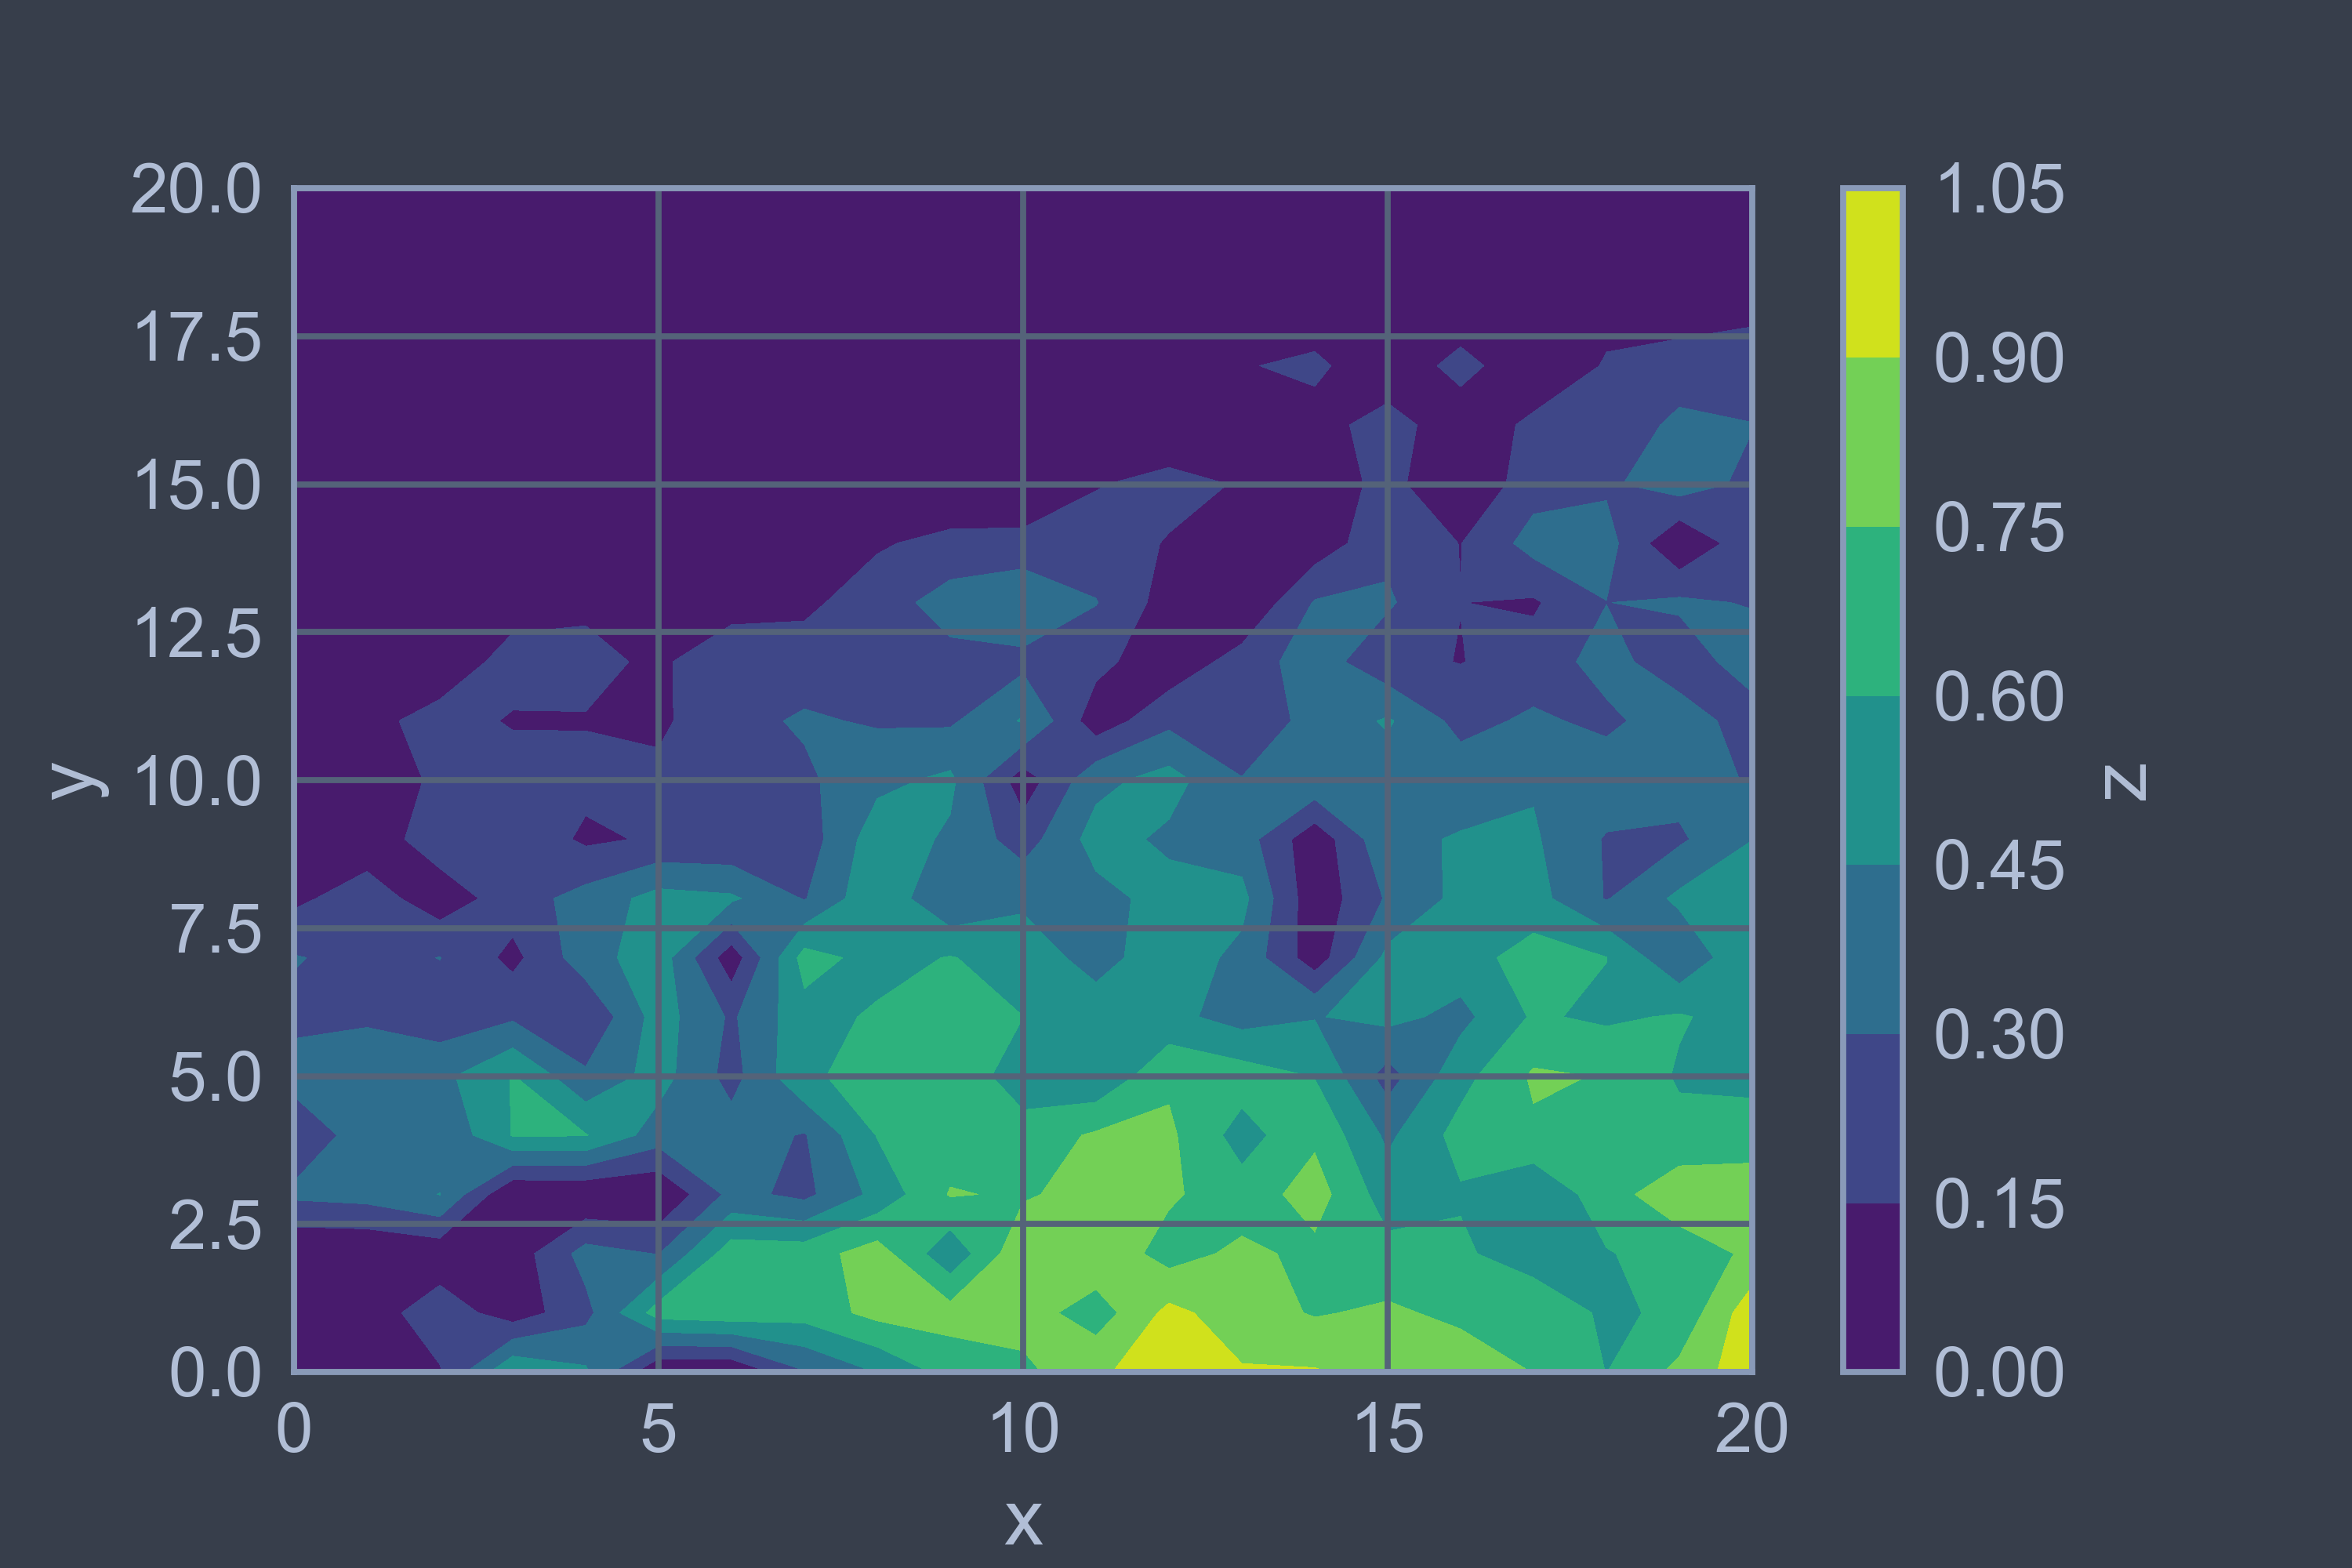
\includegraphics[width=0.4\textwidth]{terraindata.png}
    \caption{Contour plot showing the heights in the reduced terrain data set.}
    \label{fig:terraindata}
\end{figure}

The data will be standardized by removing the mean value and scaling to the standard deviation, while also being scaled such that all the values are within $[0, 1]$. 

\section{Method}

\subsection{Logistic Regression}

When we want to predict the outcome of a dataset to a specific class, such as true or false, a logistic regressor is a possible choice of machine learning model. The logistic regressor produces an outcome which can be interpret as the likelihood of a certain class being true. This means that a logistic regression model is not explicitly a classifier, but it can be used for classification by observing the produced likelihoods and choosing a cutoff percentage which decides what class the outcome should be in. Suppose we then have some data $X \in \mathbb{R}^{n \times p}$ where $n$ is the number of samples and $p$ is the number of predictors/features, while we also have the target data $y \in \mathbb{R}^n$ which contains values of either $0$ or $1$, depending on whether the outcome is true of false. While it is possible for regressors to predict more classes, since the data to be analysed in this article is binary, we will only be looking at this case. The likelihood of the outcome from a data sample $X_{i,*}$ being true ($y_i = 1$), is then given by the logistic function function of the dot product between some parameters $\beta$ and the data. I.e.

$$p(y_i = 1|X_{i,*} \beta) = \frac{exp(X_{i,*} \beta)}{1 + exp(X_{i,*} \beta)},$$

where $\beta \in \mathbb{R}^p$ are the coefficients which characterizes the logistic regression model. The probability of the outcome being in the other class is then

$$p(y_i = 0|X_{i,*} \beta) = 1 - p(y_i = 1|X_{i,*} \beta).$$


To create the best model with the highest prediction accuracy, we then need to optimize the coefficients $\beta$ such that the error of the prediction is as small as possible. To do this, we first need to define a cost/loss function. Using the Maximum Likelihood Estimation principle, it can be shown (\cite{MHJ_LogReg}) that maximizing the likelihood is the same as minimizing the so-called cost-entropy function, given by

$$C(\beta) = -\sum_i^n \left] y_i(X_{i,*} \beta) - log(1 + exp(X_{i,*} \beta))\right].$$

This means we need to find the $\beta$-values which minimizes this function. The cross-entropy is a convex function, which means any local minimum is a global minimum, and we can therefore assure that we will reach the optimal parameters by following the negative gradient. Differentiating the cross-entropy with respect to the coefficients $\beta$ we get

$$\frac{\partial C(\beta)}{\partial \beta} = X^T (p - y)$$

where $p$ are the fitted probabilities $p(y=1)$ and $y$ is the target outcome. Using stochastic gradient descent with minibatches, the optimal parameters can then be iteratively computed as

$$\beta \rightarrow \beta - \eta \sum_{MB_j} \frac{\partial C(\beta)}{\partial \beta} = \beta - \eta \sum_{MB_j} X_{i,*}^T (p_i - y_i) $$

where $MB_j$ is minibatch no. $j$, picked at random from the minibatch pool. 

As previously noted, the logistic regressor is not automatically a classifier, as the output is a continuous variable $p \in [0, 1]$. Since this value is the likelihood of the outcome being true, we can then make a classification by choosing the largest value in the set (1-p, p), where $1-p$ represents the likelihood of the outcome being false. I.e.,

$$\hat{y} = \max{\left( 1-p, p \right)}.$$

Where $\hat{y}$ will the set to $0$ or $1$ depending on which is the largest value. 

\subsection{The Neural Network}

The type of neural network to be implemented and studied in this article is the multiplayer perceptron (MLP). This network has an architecture consisting of a number of layers consisting of a n input layer, a number of hidden layers, and an output layer. Each of the layers consists of a number of nodes, whereas the first (input) layer has the same number of nodes as features in the data set and the output layer has a number of nodes equivalent to the number of possible outcomes, while the hidden layers have a varying number of nodes, and is one of the parameters of the MLP model. In order to ensure that all nodes contain values on the same scale, their inputs are passed through an activation function, such as the sigmoid function, which outputs a value between 0 and 1. In the hidden layers, each node contains a weighted sum of all the activations on the previous layer, with each neuron having a set of weights and biases that are unique to that neuron. Mathematically, the value held by a neuron $k$ in a hidden layer $l$ is given as

$$z_k^l = \sum_{i=1}^{n^{l-1}} w_{i,k} a_i^{l-1} + b^l_{i,k},$$

where $n^{l-1}$ is the number of neurons in the previous layer, and $w^l_{i,k}$ and $b^l_{i,k}$ are, respectively, the weights and biases associated with neuron $k$ in layer $l$. The activation of neuron $k$ in layer $l$ is then given by

$$a^l_k = f(z^l_k),$$

where $f$ is an activation function whose output is in the domain $[0, 1]$. By grouping the activations in a layer $l$ into a vector $a^l \in \mathbb{R}^{n^l \times 1}$, we can also create a matrix $w^l \in \mathbb{R}^{n^l \times n^{l-1}}$ containing the weights associated with each neuron, and a vector $b^l \in \mathbb{R}^{n^l \times 1}$ which holds the biases for each neuron in the same layer. This means we can write the activations in layer $l$ as 

$$a^l = f(z^l),$$

where

$$z^l = w^l a^{l-1} + b^l$$

is the \textit{weighted input} in all the neurons in layer l. Note that the input layer is only the activation of the input data, i.e.,

$$a^1 = f(x)$$

where $x$ is a vector $x \in \mathbb{R}^{n_f \times 1}$ containing the input data from one sample in the data set, with $n_f$ denoting the number of features/predictors in the data set. The output of a network with a total of $L$ layers is then the activation in layer $L$;

$$output = a^L = f(w^L a^{L-1} + b^L)$$

To exemplify this, assume we have a data set with 25 features, two possible outcomes (binary), and one hidden layer with 10 neurons. The network is then structured as shown in table \ref{tab:MLP_examp}.

\begin{table}[] \centering
\begin{tabular}{ll|l|l|l|l|}
\cline{3-6}
                                     &                   & \multicolumn{4}{c|}{Dimensions}                                                                 \\ \hline
\multicolumn{1}{|l|}{\textbf{Layer}} & \textbf{\# nodes} & \textbf{activations (a)} & \textbf{weighted sum (z)} & \textbf{weights (w)} & \textbf{bias (b)} \\ \hline
\multicolumn{1}{|l|}{1}              & 25                & $25 \times 1$            & $25 \times 1$             & N/A                  & N/A               \\ \hline
\multicolumn{1}{|l|}{2}              & 10                & $10 \times 1$            & $10 \times 1$             & $10 \times 25$       & $10 \times 1$     \\ \hline
\multicolumn{1}{|l|}{3}              & 2                 & $2 \times 1$             & $2 \times 1$              & $2 \times 10$        & $2 \times 1$      \\ \hline
\end{tabular}
\caption{Structure of an example MLP network with one hidden layer.}
\label{tab:MLP_examp}
\end{table}

Similar to other models in machine learning, the neural network needs to optimize certain parameters in order to produce accurate predictions. The parameters in the case of an MLP are the weights and biases. These values can be thought of as the ability of each neuron to recognize certain features in the data, which, for example in the case of recognizing digits from handwriting, could be recognizing certain shapes (lines or circles) in the digits. In order to optimize the the parameters, the method of backpropagation with be implemented. This algorithm works by computing the error in the output of the network (activation in layer L), adjusting the weights and biases in this layer, before repeating this for the all the preceding layers until layer number 2. In this way, the error in the prediction is \textit{propagated} backwards through the network such that the weights and biases for all the neurons in all the layers can be adjusted to make a better prediction. Before delving into the algorithm itself, we first need to define the cost/loss function for the network, which will give us the error in the prediction. Since we will apply the network to both classification and regression analysis, we will need two cost functions. For regression, we will be utilizing the mean squared error function, given as

$$C^{MSE} = \frac{1}{2n} \sum_x (y(x) - a^L(x))^2,$$

where $n$ is the total number of data sets $x, y$, $y(x)$ is the desired outcome, and $a^L(x)$ is the activation in the final layer (output of the network) with $x$ as input. Meanwhile, for classification we will, as in the logistic regression model, apply the cross-entropy cost function, which is now given as

$$C^{CE} = -\frac{1}{n} \sum_x \left[y \ln{a^L} + (1 - y)\ln{1 - a^L}\right].$$

As the cost functions gives us the error in the model for given parameters ($b$ and $w$ in case of the neural network), we essentially need to alter these parameter such that the cost function is minimized. In other words, we need to find a minimum of the function. As the cost function is often a many-dimensional function, there is no analytical solution to this problem, however we know that, for a multi-variable function, the function decreases the most (fastest) by stepping in the direction of the negative gradient. We can therefore optimize the parameters by computing the gradients of the cost function and changing the parameters proportionally to the negative resulting gradient. This is called gradient descent, and while there are many different approaches to this optimization algorithm, this article will focus on the \textit{stochastic gradient descent}-method. This is a method which approximates the gradient by taking advantage of the fact that the cost functions can be written as sums over individual data points, i.e.,

$$C = \sum_x c(x),$$

which is true for both the quadratic and cross-entropy cost function. The true gradient is then approximated by calculating the gradient on a randomly shuffled group of data points, called minibatches, and summing the resulting gradients. The new parameters are then computed as

$$\beta \rightarrow \beta - \eta \nabla_\beta C.$$

Here $\nabla_\beta C$ is the sum of gradients calculated over the data points in one minibatch $MB_j$, such that

$$\nabla C = \sum_{i \in MB_j} \nabla_\beta c (x_i)$$

where $j$ is chosen randomly among the total amount of minibatches. The parameter $\eta$ denotes the learning late, and affects how far in the direction of the gradient we want to step. A large value of $\eta$ can cause multiple overshoots, resulting in a longer time taken in finding the minimum, while a too small value of $\eta$ could result in such small steps that the algorithm never converges to a minimum within a given threshold within the maximum number of iterations. Therefore, the learning rate is a parameter which needs to be tuned such that a minimum is reached within a reasonable amount of iterations. 

With the method of stochastic gradient descent for optimizing the parameters in the cost function, we can return to the idea of backpropagation. For reason to be shown later, We define the quantity

$$\delta^l \equiv \frac{dC}{dz^l}$$

as the error of the neurons in layer $l$, and

$$\delta^L = \frac{dC}{a^L} f'(z^l)$$

as the error of the neurons in the output layer. This can also be written as

$$\delta^L = \nabla C_a \odot f'(z^l)$$

where $\nabla C_a$ is the gradient of the cost function with respect to the activation, and $\odot$ denotes the Hadamard product, or element-wise multiplication. Knowing the error in output layer, we can then apply the weights in the previous layer to this error, in order to produce the error in the output of this layer. By then applying the derivative of the activation function, this error becomes the error in the weighted input of the layer. In other words, the error from the output layer is propagated backwards through the previous layers in the networks, such that each layer can adjust its own weights in order to minimize the network output layer. This can be written as

$$\delta^l = \left[((w^{l+1})^T \delta^{l+1}\right] \odot f'(z^l).$$

The purpose of backpropagation is to locate the minimum of the cost function by computing its gradients. It can be shown that the gradient of the cost function with respect to the biases in layer $l$, $\beta^l$ is given by

\begin{equation}\label{eq:nablac_beta}
    \frac{\partial C_{\beta^l}}{\partial \beta^l} = \delta^l,
\end{equation}

which shows the reason behind the expressions for the $\delta$-errors. Similarly, the gradient of the cost function with respect to the weights in layer $l$, $w^l$ is defined as

\begin{equation}\label{eq:nablac_w}
    \frac{\partial C_{w^l}}{\partial w^l} = (a^{l-1})^T \delta^l.    
\end{equation}

Knowing the gradients of the cost functions, the optimal values for the weights and biases can then be iteratively computed as

$$w^l \rightarrow w^l - \eta \frac{\partial C_{w}}{\partial w^l}$$

$$\beta^l \rightarrow \beta^l - \eta \frac{\partial C_{\beta}}{\partial \beta^l}.$$

The backpropagation algorithm can then be presented:

\begin{enumerate}
    \item Compute the activation in the input layer $a^1$
    \item Compute the weighted inputs $z^l$ and activations $a^l$ for all layers $l \in [2, L]$ where $z^l = w^l a^{l-1} + b^l$ and $a^l = f(z^l).$
    \item Compute the error in the output layer $\delta^L = \nabla C_a \odot f'(z^l).$
    \item Compute the gradients of the cost function using \ref{eq:nablac_beta} and \ref{eq:nablac_w}.
    \item Update the weights and biases with the produced gradients.
\end{enumerate}

By utilizing stochastic gradient descent, this algorithm will be applied to all the minibatches in random order, 

As with many other machine learning models for predicting data, overfitting the neural network is a potential problem when training the model. In the case of a multilayer perceptron, overfitting happens when certain weights become too large and dominate. This results in low flexibility of the model, as the dominating weights as specialized for a specific data set, and will therefore perform poorly when predicting on new data. To avoid this, a regularization parameter can be added to the cost function. This parameter act as a penalty for the weights, preventing them from growing too large and dominating the predictions. The cost function with the added regularization term is given as

$$C \rightarrow C + \frac{\lambda}{2n}\sum_w w^2$$

Where $\lambda$ is the regularization parameter, and determines how much to penalize the weights and $n$ is the size of the data set. Since the regularization term is only dependent on the weights, the updated biases are not affected by this term. However, the new weights are now computed as

$$w \rightarrow w - \eta\frac{\partial C_w}{\partial w} - \frac{\eta \lambda}{n} w,$$

where we see that the new weights are penalized by some value determined by $\lambda$.

When using the network to make a classification prediction, a similar approach to that of the logistic regressor is required, as the output of the network are continuous variables in $[0, 1]$ (this does depend on the activation function used in the final layer, but this article will only be utilizing the sigmoid/logistic function in the output layer, and it is therefore relevant for this experiment.). The network has the same number of output nodes as there are classes in the data set. For the binary case of the classification data set to be analyzed in this experiment, the network then has two output nodes. The value at each of the output neurons can then be thought of the networks security in its prediction. For example, for the binary case, a value of $0.9$ in the first neuron indicates that the network is 90\% sure that the outcome should be 0. The classified prediction of the network is then the index of the output node with the largest value. For the case of regression, the target is one continuous variable, which means we only have one output neuron. By making sure the input data set is in the domain $[0, 1]$, we can simply use the value produced by the neuron. In the case of the terrain data to analyzed in this experiment, the network will then have two input neurons, for $(x_i, y_i)$-coordinates, followed by a number of hidden layers with a certain number of neurons, and finally with a single-neuron output layer which will correspond to the terrain height at the input coordinates. As the cross-entropy cost function is defined for the cost between two probabilities, it is not relevant for a regression model. It is therefore necessary to change the cost function to one that is more suited for continuous outcomes, as produced by regression. The cost function we will utilizing for regression is then the mean-squared error, defined as

$$C^{MSE} = \frac{1}{2n} \sum_x ||y - a^L(x)||^2$$

where $y$ are the target values and $a^L(x)$ are the predicted values with input $x$. 


\section{Results}

To determine the impact of the size of the minibatches used in the stochastic gradient descent method, the cost (error) of the logistic regressor was computed for a varying value of the learning rate and an increasingly large size of the minibatches. Using 300 data points, the error was computed with minibatch sizes of $30, 75, 150$ and $200$. The resulting error heat map is shown in figure \ref{fig:logreg_minibatch}.

\begin{figure}
    \centering
    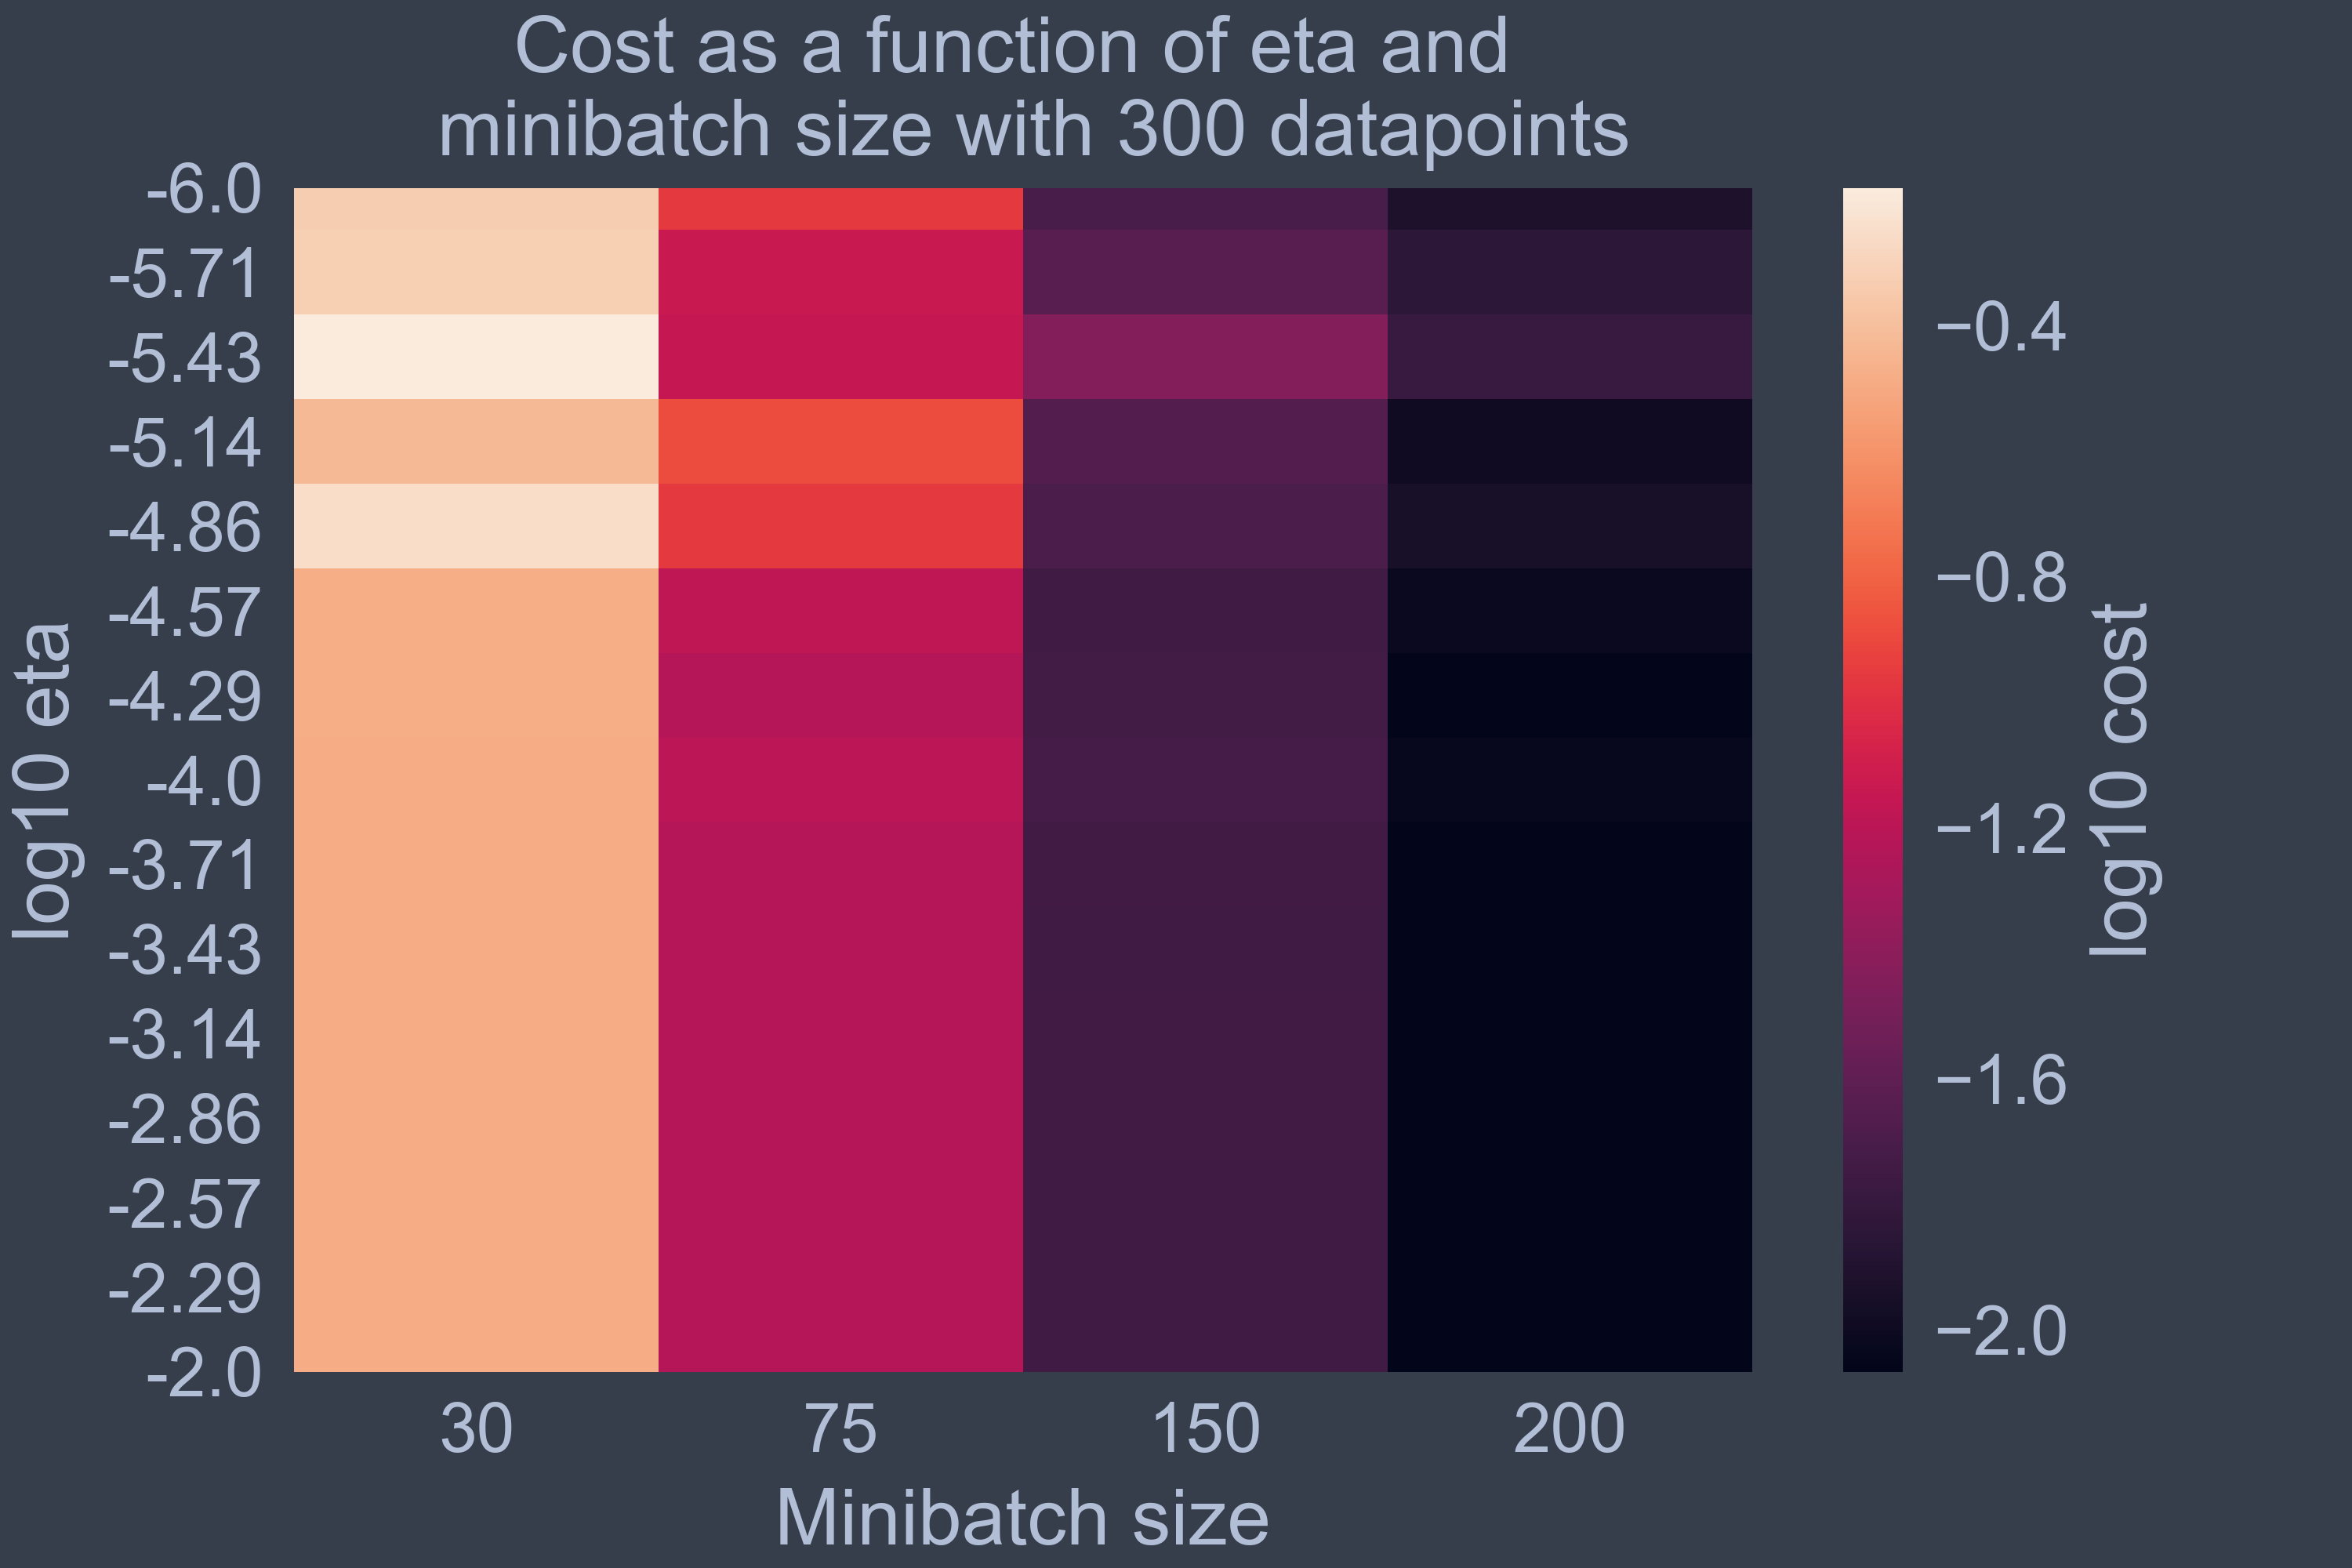
\includegraphics[width=0.5\textwidth]{cost_etas_mbsize.png}
    \caption{Cost of the logistic regression model as a function of the learning rate and minibatch size with 300 total data points.}
    \label{fig:logreg_minibatch}
\end{figure}

With a set minibatch size of $n/10$ where $n$ is the total number of samples, the logistic regressor was evaluated for a varying value of the learning rate with 3000 data points. For each learning rate value, the model was trained for 1000 epochs, and the minimum error produced on the testing set was extracted, along with the epoch number at which the minimum error was reached. This result is shown in table \ref{tab:logreg_etas}.

\begin{table}[] \centering
\begin{tabular}{|l|l|l|}
\hline
log10 $\eta$ & minimum cost & epoch no. at minimum cost \\ \hline
-3.84        & 0.72         & 1000                      \\ \hline
-3.68        & 1.12         & 1000                      \\ \hline
-3.53        & 0.65         & 1000                      \\ \hline
-3.37        & 0.66         & 1000                      \\ \hline
-3.21        & 0.65         & 1000                      \\ \hline
-3.05        & 0.65         & 796                       \\ \hline
-2.89        & 0.65         & 1000                      \\ \hline
-2.74        & 0.65         & 484                       \\ \hline
-2.58        & 0.65         & 1000                      \\ \hline
-2.42        & 0.65         & 112                       \\ \hline
-2.26        & 0.65         & 742                       \\ \hline
-2.11        & 0.65         & 563                       \\ \hline
-1.95        & 0.65         & 376                       \\ \hline
-1.79        & 0.65         & 262                       \\ \hline
-1.63        & 0.65         & 175                       \\ \hline
-1.47        & 0.65         & 29                        \\ \hline
-1.32        & 0.65         & 10                        \\ \hline
-1.16        & 0.65         & 65                        \\ \hline
-1.0         & 0.65         & 8                         \\ \hline
\end{tabular}
\label{tab:logreg_etas}
\end{table}

A plot showing the errors as a function of the number of epochs is shown in figure \ref{fig:logreg_etas_plot}. As most of the change in the cost was in the first 300/400 epochs, only this part of the results is shown.

\begin{figure}
    \centering
    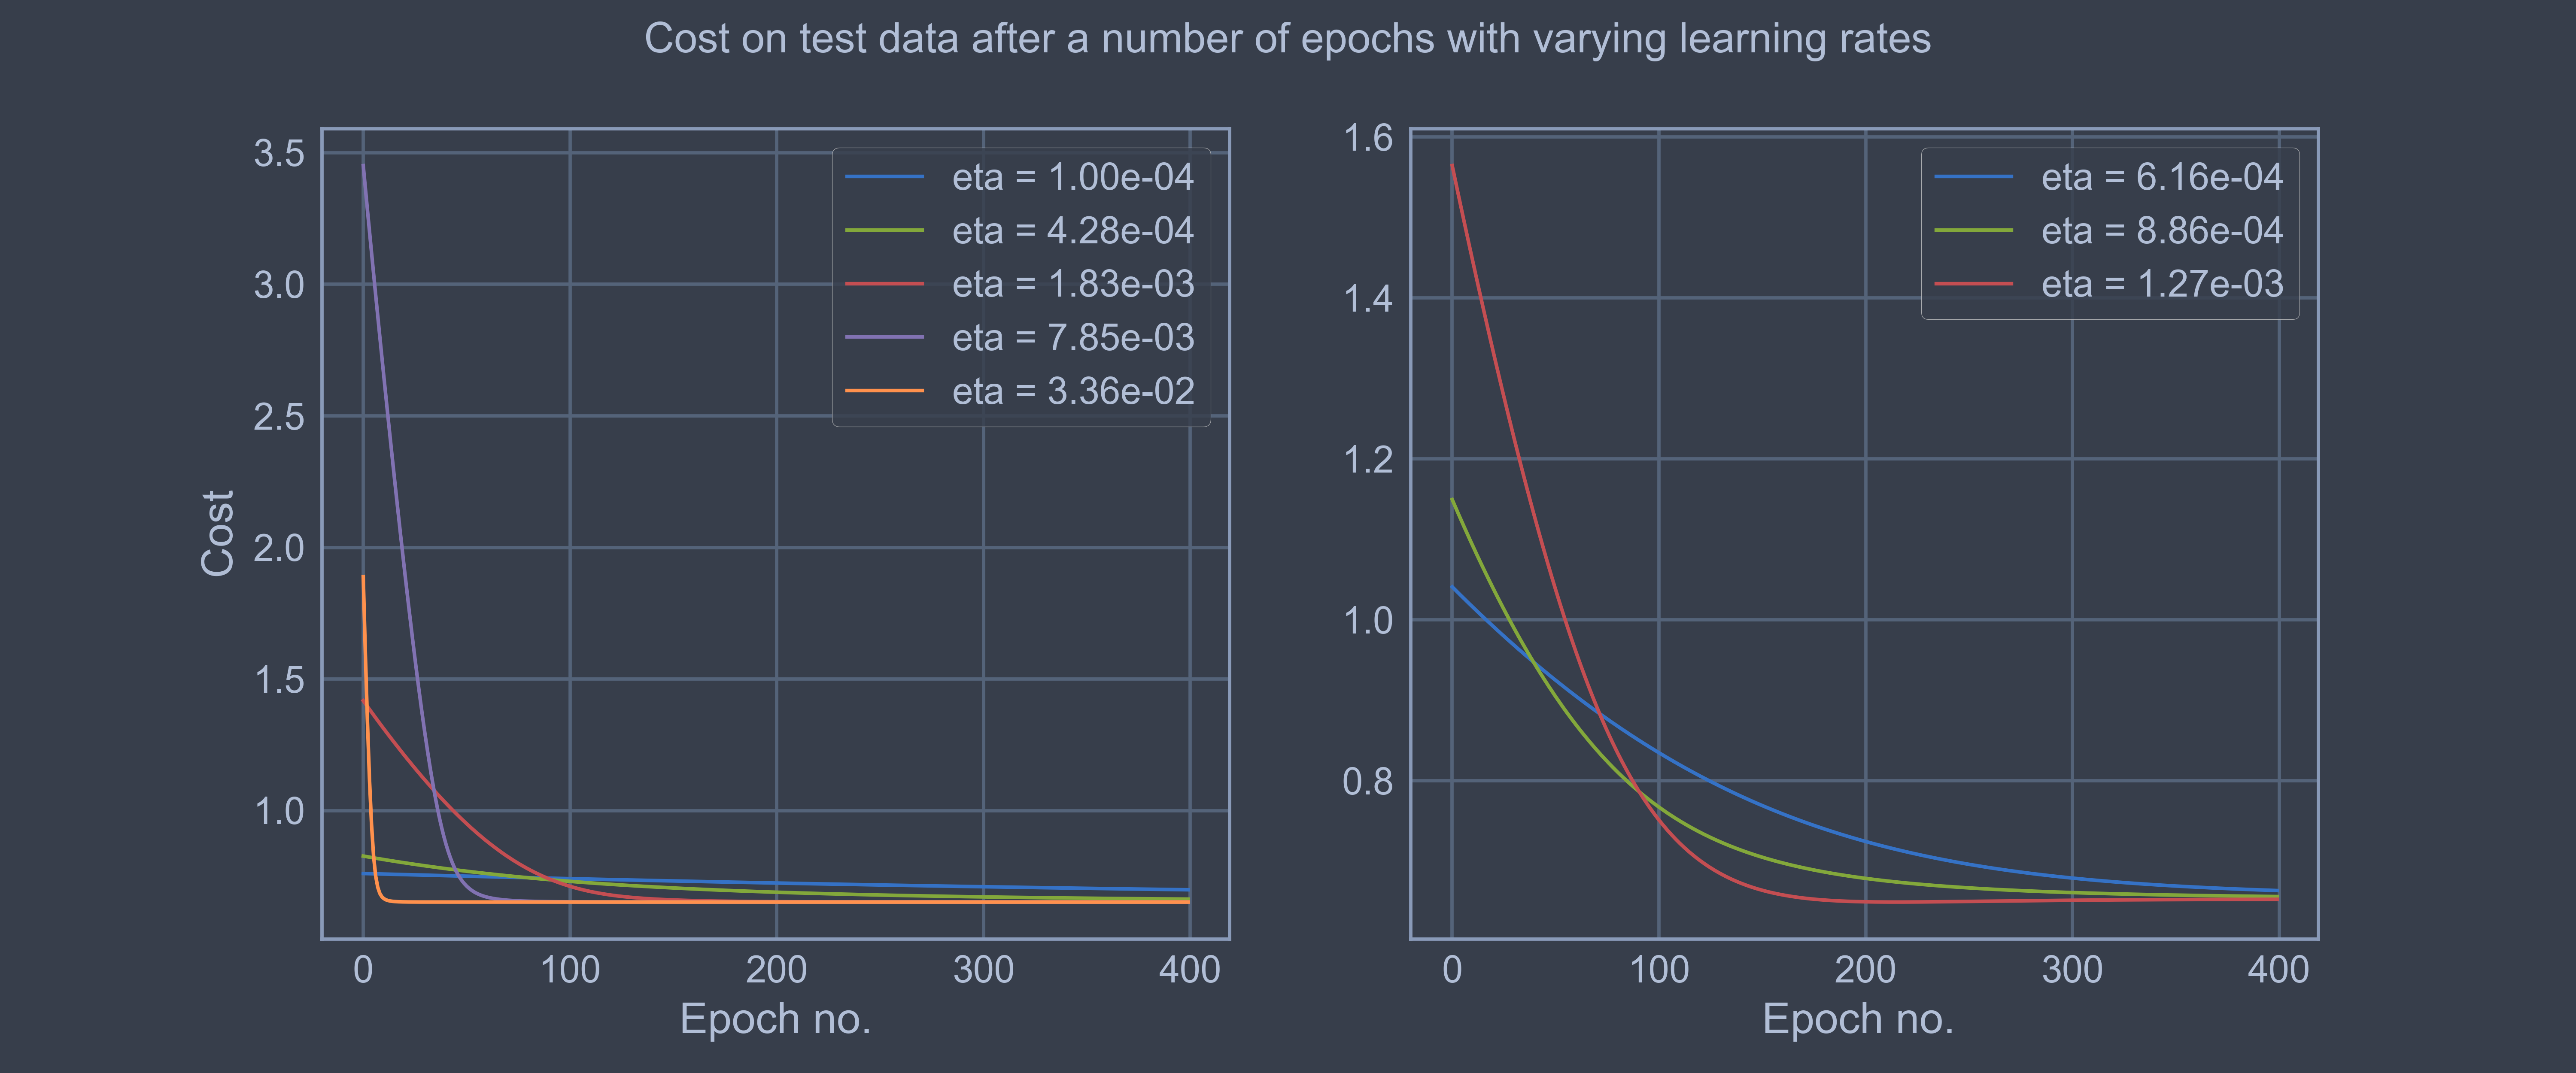
\includegraphics[width=0.8\textwidth]{logreg_learningrates.png}
    \caption{Cost on the test data as a function of epochs with varying learning rates. The rightmost plot shows a smaller selection of the curves in the left plot.}
    \label{fig:logreg_etas_plot}
\end{figure}

A value of $\eta$ and a number of epochs which produced reasonable results was then chosen, namely $\eta = 10^{-1.79}$, and $300$ epochs. The model was then trained on $80\%$ of the credit card data set, before predicting on the remaining training set. Finally, the F1 score and accuracy was computed, in addition to the CPU time taken to train the model and make the final prediction. The same procedure was performed using scikit-learns logistic regressor model, and the result of both models is shown in table \ref{tab:logreg_own_scikit}.

\begin{table}[] \centering
\begin{tabular}{|l|l|l|l}
\hline
         & Own model & Scikit \\ \hline
F1 score & 0.61      & 0.75   \\ \hline
Accuracy & 0.57      & 0.80   \\ \hline
Time [s] & 3.27 & 0.03 \\ \hline
\end{tabular}
\label{tab:logreg_own_scikit}
\end{table}

For the neural network classification, the best parameters for the network, namely the learning rate and hidden layer architecture, were located by training and validating the network on a subset of the data set ($1\%$, or 300 data points) with 300 epochs. The learning rates used were 10 equally spaced values between $10^{-6}$ and $10^{-2}$, while the layer architectures used were (including input and output layer)

\begin{itemize}
    \item (2, 2)
    \item (2, 10, 2)
    \item (2, 100, 2)
    \item (2, 10, 10, 2)
    \item (2, 100, 10, 2)
\end{itemize}

where the numbers represent how many neurons were in each layer. A result of the minimum error produced by the different combinations is shown in figure \ref{fig:neuralnet_heatmap}., 

\begin{figure}
    \centering
    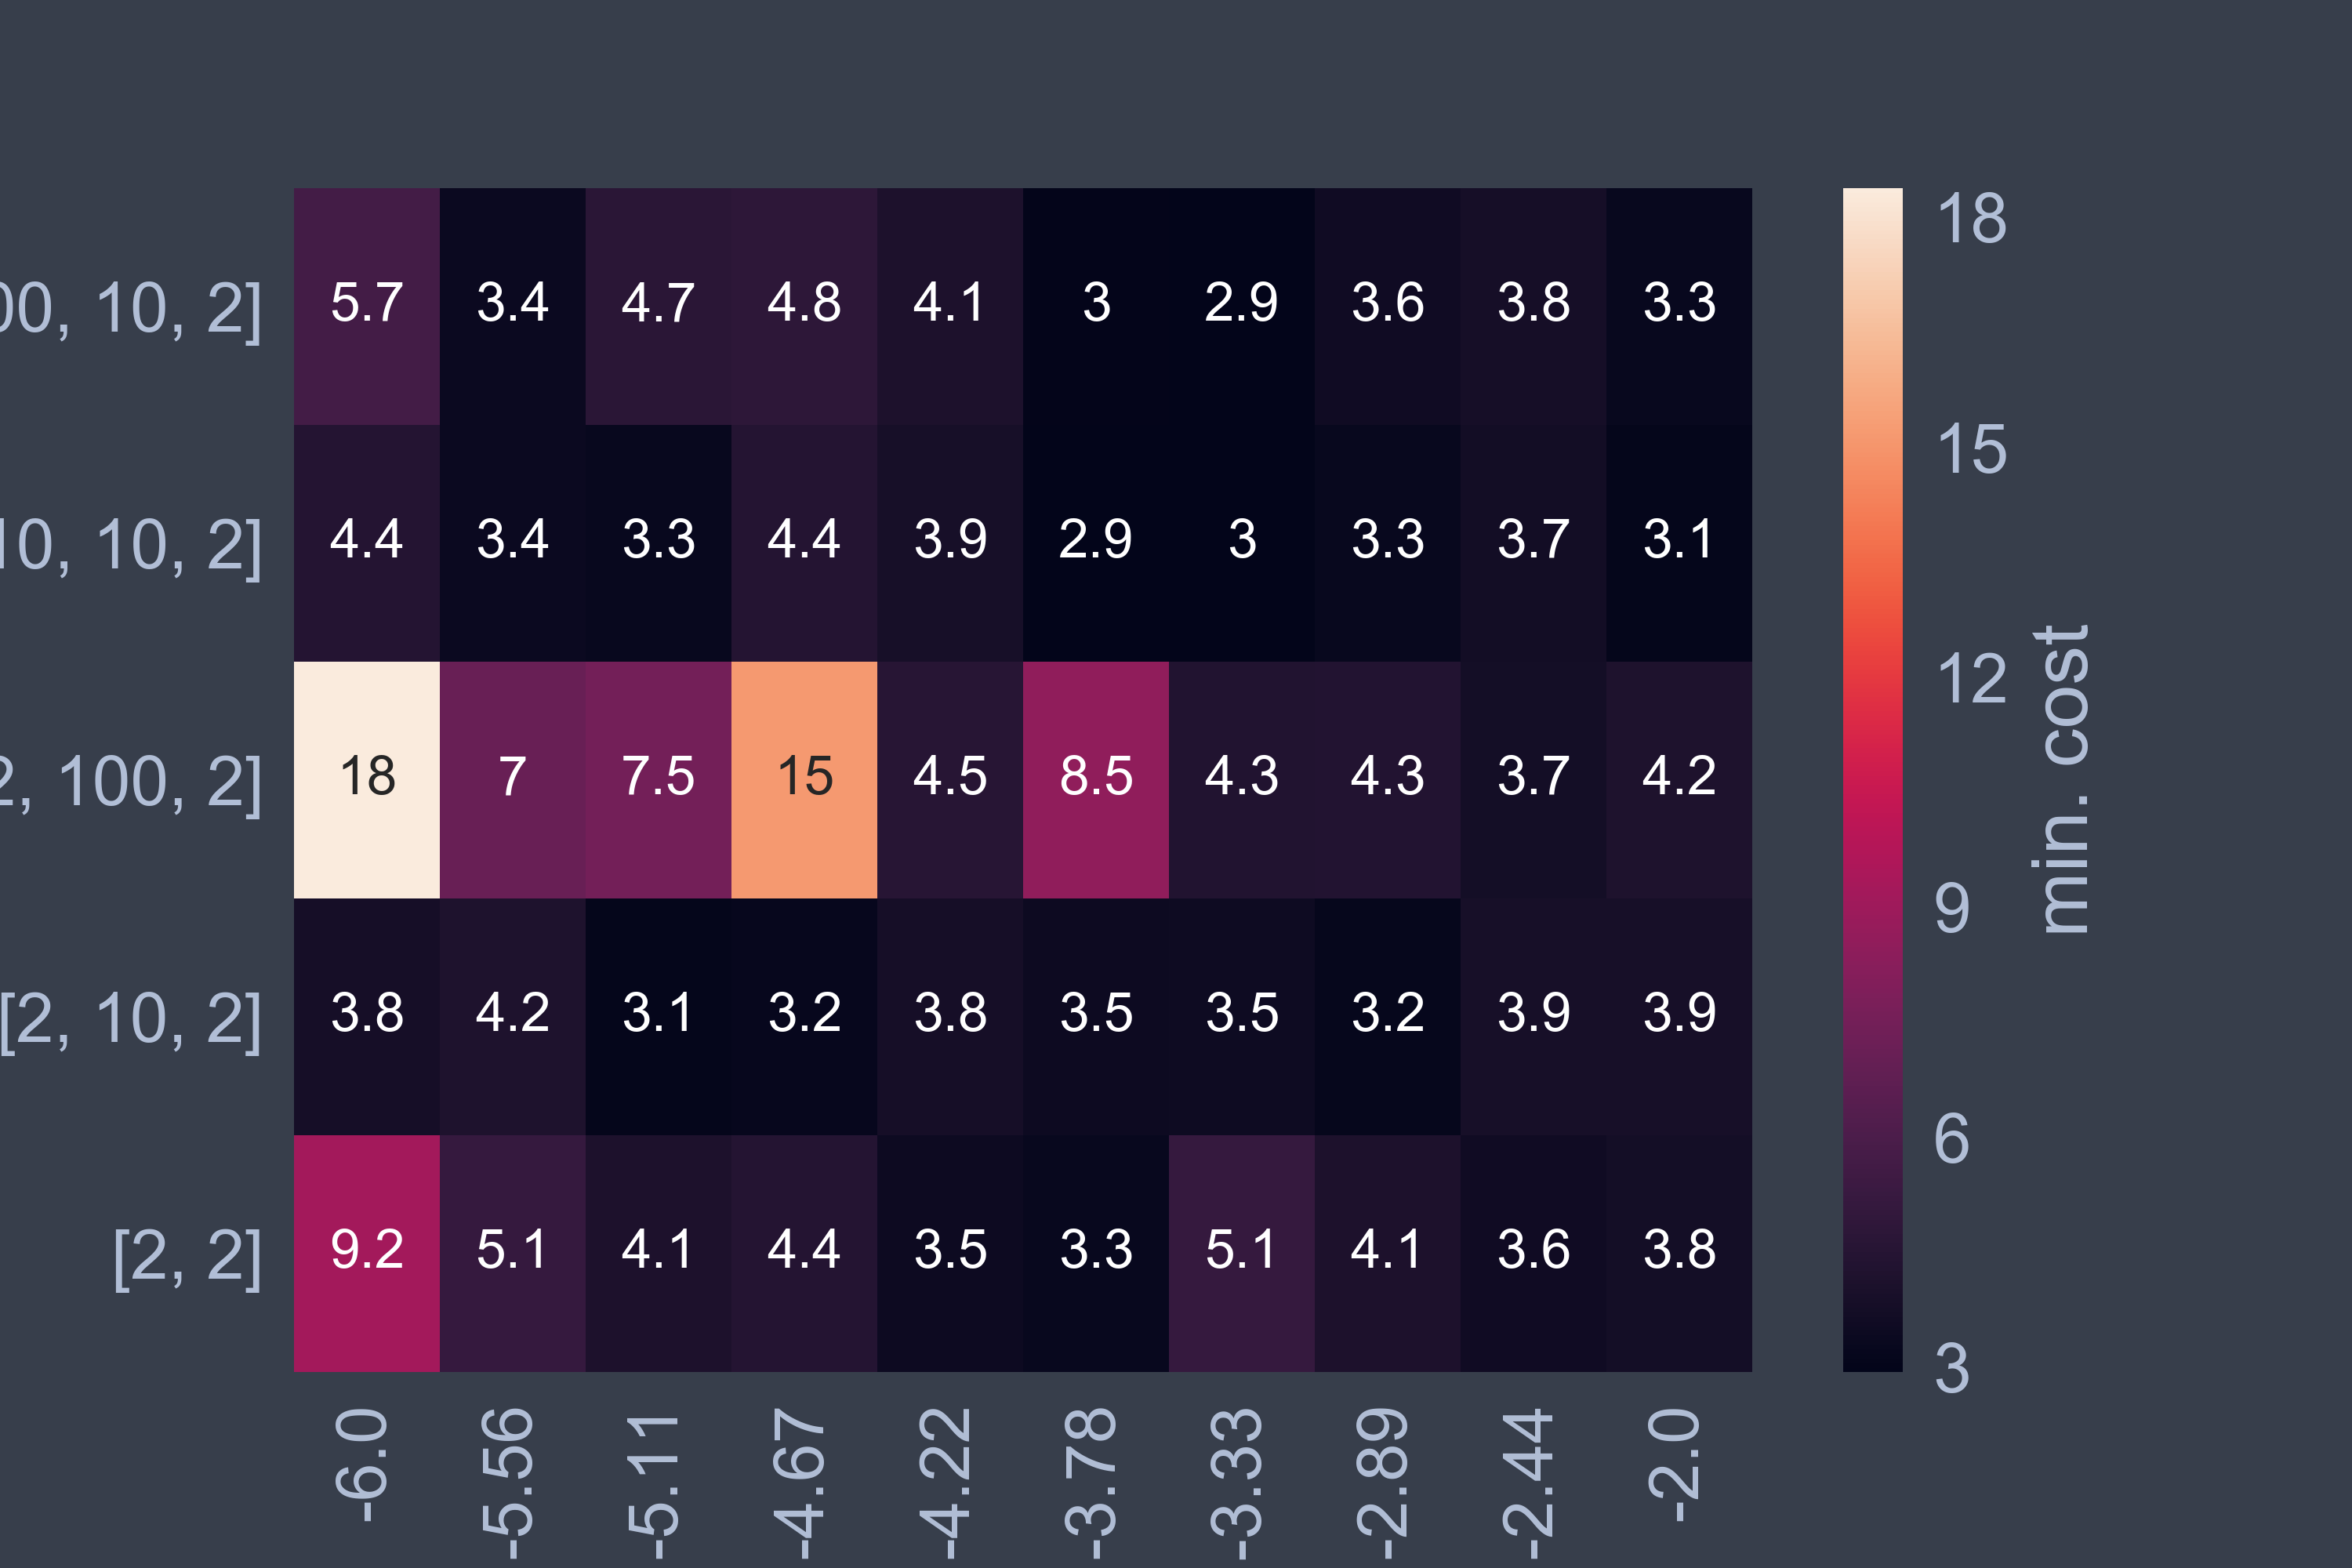
\includegraphics[width=0.5\textwidth]{neuralnet_heatmap.png}
    \caption{Caption}
    \label{fig:neuralnet_heatmap}
\end{figure}

while a figure showing the cost as a function of epochs for a selection of the learning rates, for all layers is shown in figure \ref{fig:neuralnet_cost}.

\begin{figure}
    \centering
    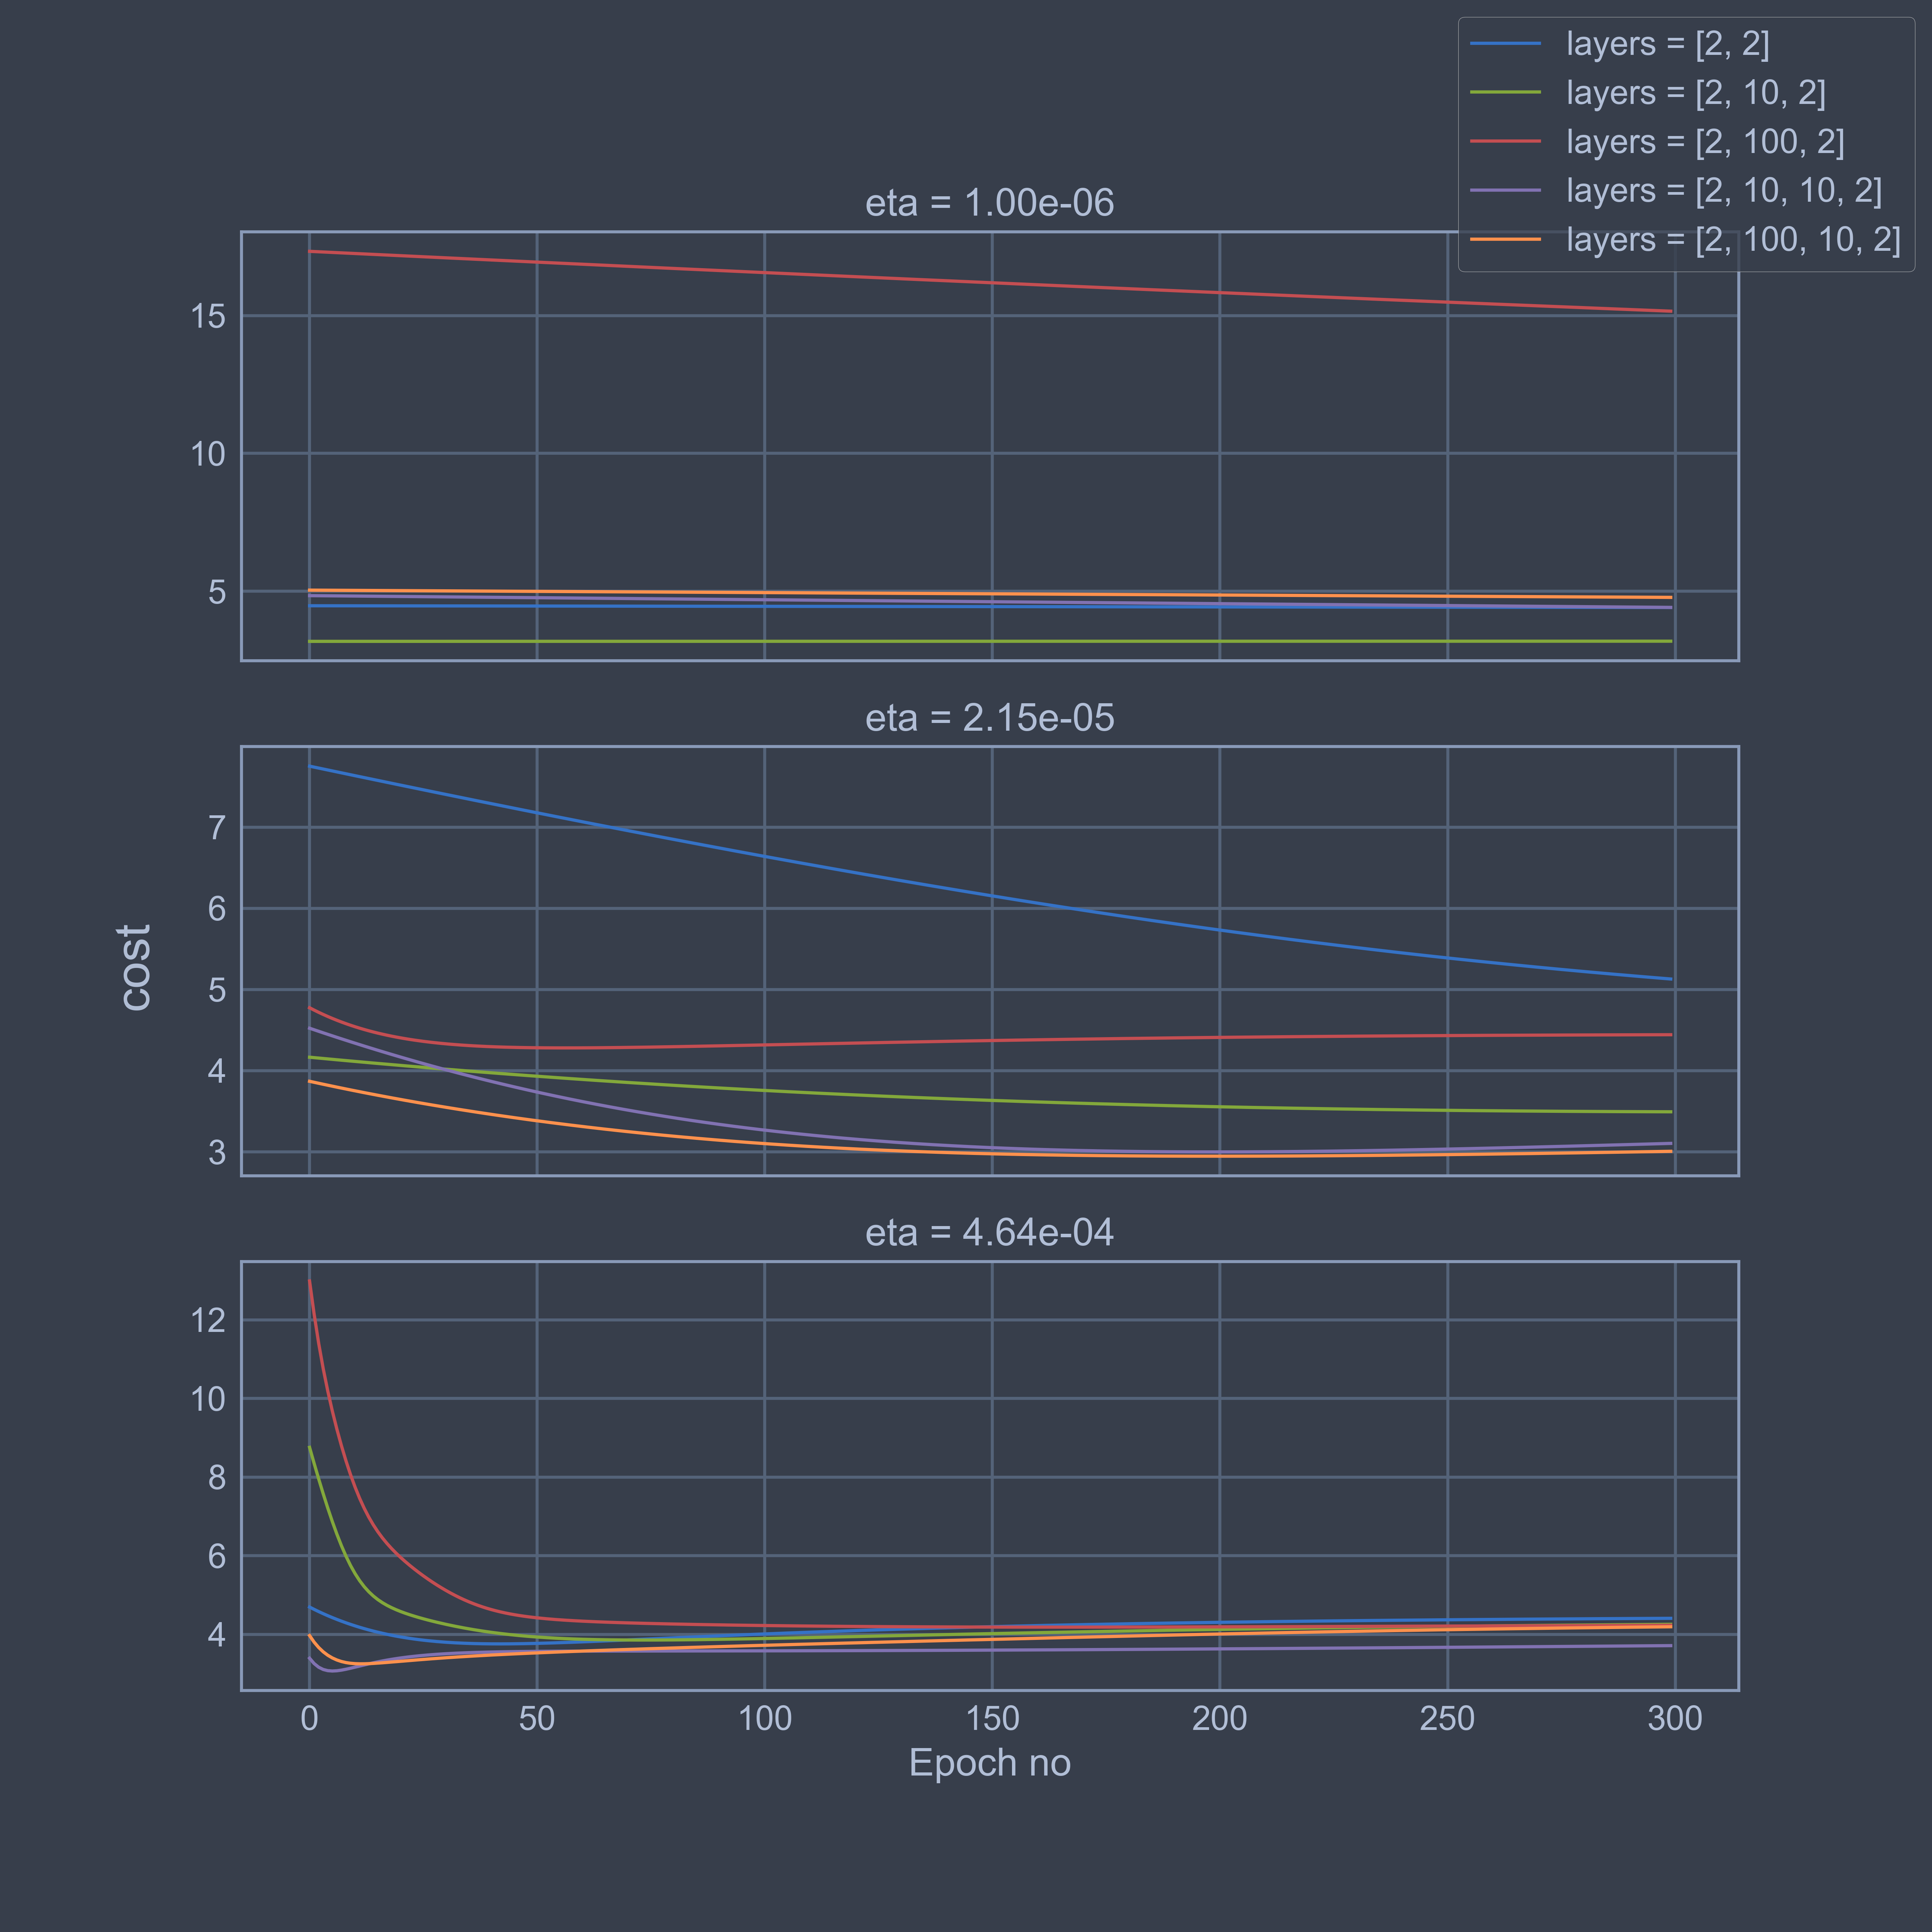
\includegraphics[width=0.8\textwidth]{neuralnet_cost.png}
    \caption{Cost (cross-entropy) on the test data from the neural network as a function of epochs, for a selection of learning rates and network architecture.}
    \label{fig:neuralnet_cost}
\end{figure}

The best combination of learning rate and layer was then chosen to as the parameters for the model which would be trained and validated on the whole data set. Using then a value of $\eta = 10^{-3.78}$, the hidden layers $(10, 10)$, and 300 epochs, the network was initialized and trained on $80\% = 24000$ of the data points, and the validated on the remaining $6000$ samples. The scores were then compared to an MLP-network from the scikit, which was initialized with the same parameters as the self-written network. The resulting score and CPU time is shown in table \ref{tab:neuralnet_own_scikit}.

\begin{table}[] \centering
\begin{tabular}{|l|l|l|l}
\hline
         & Own network & Scikit \\ \hline
F1 score & 0.88      & 0.88   \\ \hline
Time [s] & 1589 & 5.27 \\ \hline
\end{tabular}
\label{tab:neuralnet_own_scikit}
\end{table}

The neural network was used as a regressor in an attempt to predict the terrain data as visualized in \ref{fig:terraindata}. To find a suitable model, the network was initialized and trained with various combinations of the regularization parameter $\lambda$ and number of neurons in the hidden layer. Multiple hidden layers were initially utilized, but did not produce observable differences in the prediction of the model. As a result, only one hidden layer with varying number of neurons was used. The learning rate was set to $10^{-3}$ as this produced the most stable results with convergence within a reasonable amount of epochs. The mean squared error of the model on the test set was then computed and visualized in the heat map shown in figure \ref{fig:terrain_heatmap}.

\begin{figure}
    \centering
    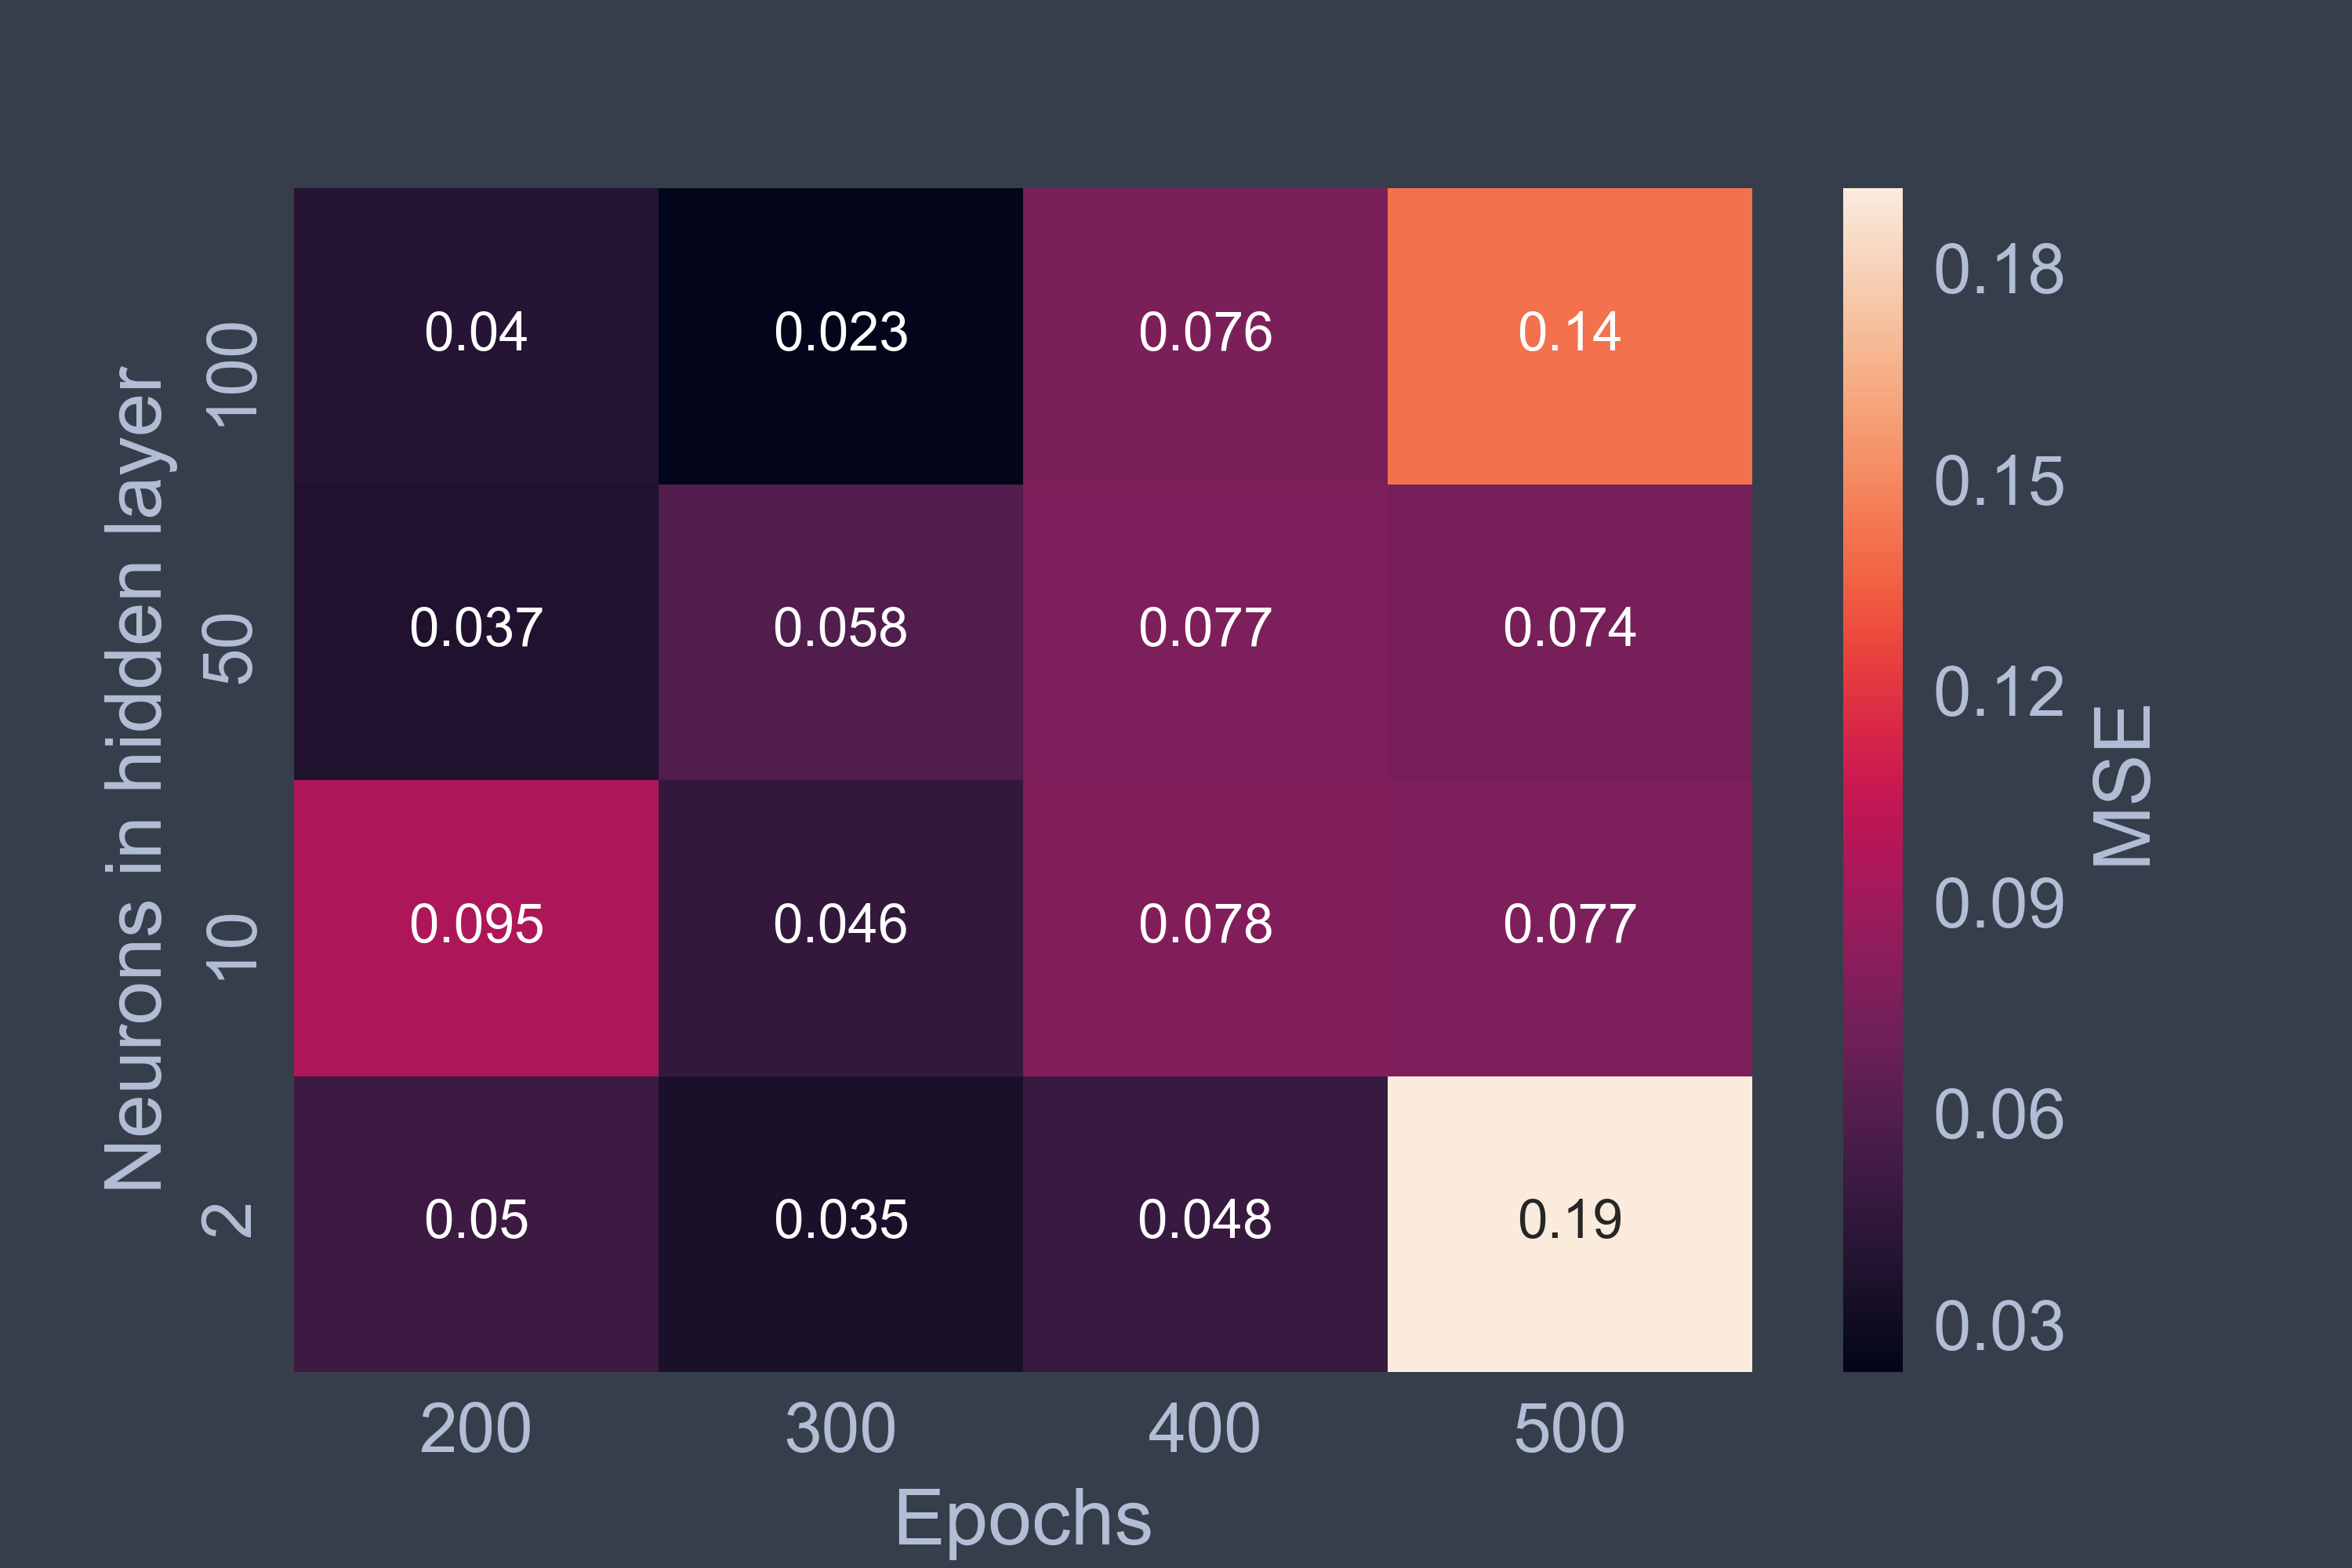
\includegraphics[width=0.7\textwidth]{terrain_heatmap.png}
    \caption{Caption}
    \label{fig:terrain_heatmap}
\end{figure}

The best combination of $\lambda$ and neurons in the hidden layer, in this case $300$ epochs with 100 hidden neurons, was then used to train the model and predict the terrain on the whole data set. A contour plot of the result, alongside the original data, is shown in figure \ref{fig:predicted_terrain}.

\begin{figure}
    \centering
    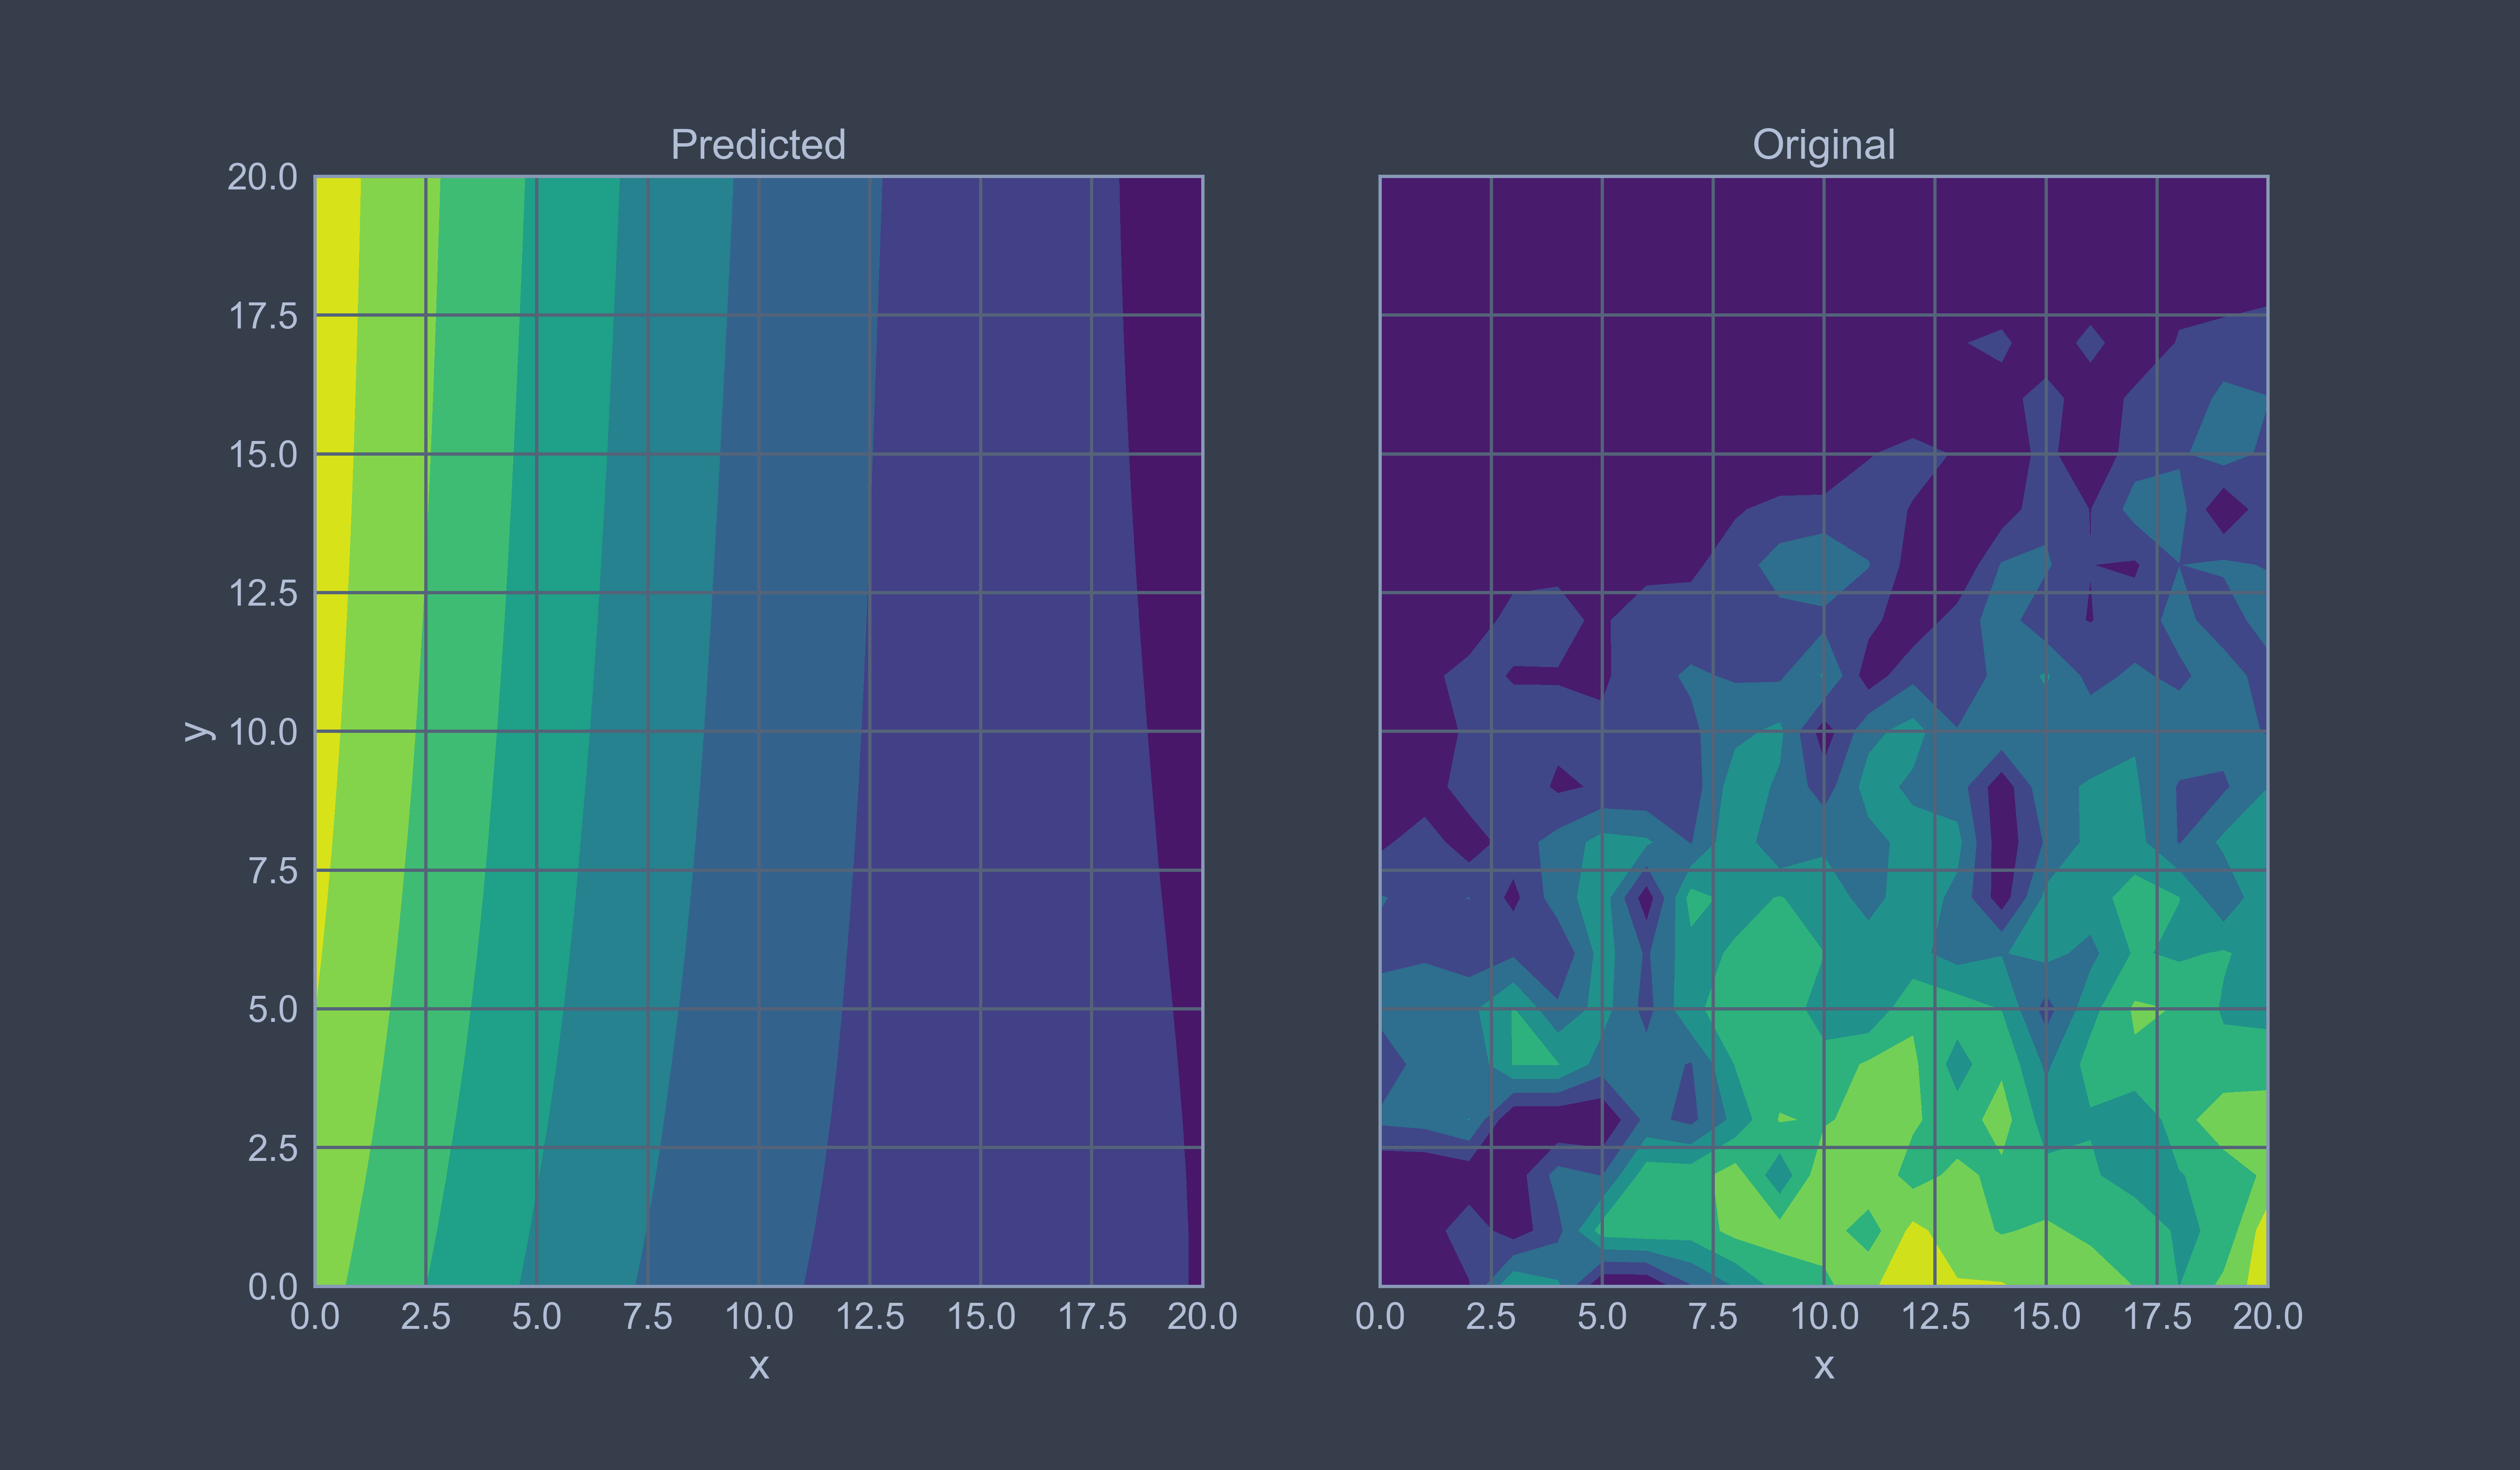
\includegraphics[width=0.8\textwidth]{predicted_terrain.png}
    \caption{Predicted terrain height vs original input data. Lighter areas indicate higher terrain.}
    \label{fig:predicted_terrain}
\end{figure}

\section{Discussion}

The heat map of the error produced by the logistic regressor with varying minibatch sizes (figure \ref{fig:logreg_minibatch}) shows us that the size of the minibatch greatly impacts the optimization of the parameters in the model, with a larger minibatch producing smaller errors. This is not surprising, as the idea of using minibatches is to reduce the computational cost of calculating the gradient. By using minibatches, the minimum localizer "jumps" around, compared to gradient descent on the whole data set, which slowly follows the gradient directly to the minimum. However, the 'jumps' are not always in the correct direction of the global minimum. The parameters stumble around, but generally follows the path to the minimum, however if the sizes of the minibatches are too small, there will be many small jumps, which will stumble more than when computing the gradient on larger batches. As a result, convergence will require more epochs to be reached. At the same time, it computationally cheaper to calculate the many small gradients than fewer large ones, which means that the higher amount of epochs might not necessarily require a larger CPU time. In this experiment, computational efficiency was not one of the topics, and the minibatch size was therefore set to $10\%$ of the original data set (training data).

The results in table \ref{tab:logreg_etas} show that for the smallest values of $\eta$, the optimal parameters do not converge within 1000 epochs, indicating that the learning rate is small enough such that more epochs are required for convergence. However, we see that for the majority of $\eta$-values, convergence was reached at a training cost value of $0.65$. We see that generally the amount of epochs required to reach this minimum decreases as the learning rate increases. Table \ref{tab:logreg_own_scikit} shows then the result of training the logistic regressor model using a $\eta$-value of $10^{-1.79}$ and 300 epochs. The self written model produced an f1 score of $0.61$ and an accuracy of $0.57$, while the logistic regressor from scikit produced both a larger f1 score and a higher accuracy. It is not surprising that the scikit logistic regressor performs better than the self-written model, however this is a significant difference which does indicate a larger systematic error in the self-written code. Most likely, the best parameters have not been located when performing a grid search of the optimal values and a more thorough search of the best learning rate and number of epochs should be considered. However, it this article did choose the parameters which resulted in the smallest cost, but there is reason to believe there is a systematic error in the code itself, due to the fact that the model converged at a cost value which not close to $0$, which indicates that something is preventing the model from increasingly optimizing the parameters. 

While the accuracy score is, as previously mentioned, not a good metric for evaluating the model, it still provides interesting topics for discussion. We see that the scikit has an accuracy of $80\%$, which indicates that the model predicted a majority of values of $0$, as the data set contains around $80\%$ zero values. This shows why this biased data set is problematic. The (scikit) model scored high in its validation, but it is extremely biased, and would perform poorly on new data which is more symmetric than the dataset in question. This is, of course, only the case is the data set is not an accurate representation of the rest of the credit card clients. Nevertheless, it is worth keeping in mind that while the model scores high, it is biased in that it is trained on a majority of one class, meaning that it would perform significantly worse if a new data set was more symmetric with a higher percentage of samples who defaulted. With this in mind, it is possible to speculate that the self-written model, with its smaller f1-score and accuracy could potentially be a better model if new, more symmetric data was introduced. This is only speculation in this article, but could be studied by actively choosing a symmetric subset of the data set and validating the model on this.


The cost heatmap of the neural network (figure \ref{fig:neuralnet_heatmap}) shows some patterns, in that the cost is generally higher for the first (smallest) learning rate, indicating that with this learning rate, 300 epochs is not enough for the model to converge. This is also shown in the top plot in figure \ref{fig:neuralnet_cost}, where we see that, for all layer combinations, the error does not seem to have reached a minimum. In the middle plot of the same figure, we do see that the gradient descent seemingly converges for the network with two hidden layers, after $\approx$ 200 epochs. Finally, in the bottom plot, it appears that all layer combinations converge after certain epochs, with the two networks with one hidden layer converging slower then the others. For the dual-hidden layer network, the error starts significantly smaller than the single hidden layers, before decreasing even further, and then increasing slightly again. This could indicate overfitting, however it is unknown why more hidden layers would produce overfitting faster than only one hidden layer. Table \ref{tab:neuralnet_own_scikit} shows the result of initializing the network with the parameters of the best-performing models, name $eta = 10^{-3.78}$, 300 training epochs, and two hidden layers with 10 neurons each. The most striking feature is that both the self-written model and the MLP-network from scikit produced the exact same f1-score. This is not necessarily surprising, as the scikit MLP network was initialized with the same parameters as the self-written module, namely with an SGD solver, a logistic activation function, 300 training epochs, and the same learning rate. This is, however, a reassuring result that the self-written network does work as intentional. Upon further inspection, it was observed that the high f1-score was a result of the two models predicting only values of $0$, which is not necessarily a bad thing for this specific data set. By training the models on $80\%$ of one class, it will, as already discussed, be biased for this class. 

Based only on the f1-score, it is easy to say that the neural network outperformed the logistic regression model in the case of classification. However, it must be noted that the self-written neural network used almost $500$ times as much CPU time as the self-written logistic regressor, while the scikit MLP used $165$ times the CPU time of the scikit logistic regressor, while only producing a $0.1$ higher f1 score. This extreme difference should then be taken into account when choosing the the model data mining. 

The question then is why did the neural network perform so much better than the logistic regressor. In many ways, the logistic regression model can be thought of as a no-hidden-layer neural network, as the model takes the same amount of inputs as there are features in the data set, sums the weighted inputs, and applies the logistic function. A network with some hidden layer, then, contains more ability to adjust itself to the data. For the logistic regression model, only two parameters can be adjusted such that the model can produce accurate results, while a neural network can contain hundreds of parameters that can act as identifiers for certain features in the data. It is then not surprising that a neural network outperforms a simple logistic regression model, especially considering the significantly higher computational cost. 

It should be noted that the best possible MLP classifier has not necessarily been found, as there are multiple combinations of gradient descent solvers, activation functions, learning rates, layer architectures, and much more which should be further studied.

The result of the terrain data prediction gives us pretty good indication of the neural networks ability to perform regression. The contour plot of the predicted terrain, shown in the leftmost plot in figure \ref{fig:predicted_terrain}, shows that the network is able to recognize the general features of the landscape. It predicts an area of low height in the domain of large $y$-values and small $x$-values, with a gradual increase in height as $x$ is increased and $y$ is lowered. We observe that this is somewhat similar to the general shape of the terrain in the original data set. 

\begin{figure}
    \centering
    \includegraphics[width=0.8\textwidth]{terrain_result.png}
    \caption{Caption}
    \label{fig:linreg_terrain}
\end{figure}

When compared to the terrain predicted using a linear regression model with a polynomial of degree 5 (figure \ref{fig:linreg_terrain}), we see that this model was substantially better at predicting specific features in the terrain than the neural network. The reason for this large difference is unknown. It was assumed by the article that having a network with a large amount of hidden layers, or one hidden layer with a large amount neurons would be able to accurately reproduce the terrain, perhaps even better than then linear regressor, due to the large amount of weights and biases that can be adjusted for the different coordinates on the meshgrid. However, this was not observed, as a predicted terrain similar to that in figure \ref{fig:predicted_terrain} was produced for up to 5 hidden layers. Based on the results, then, one could conclude that the neural network is not a good candidate for regression, but due to the author's uncertainty in why this is the case, this is not an answer with a high confidence.

\section{Conclusion}

The results from both the classification and regression using a logistic regressor and a neural network show that the neural network outperforms the logistic regression model in terms of accuracy, but it is, however, significantly slower. The self-written logistic regression code did you produce satisfactory results, but the abovementioned conclusion can be made using the results from the scikit-learn module. For regression, the neural network was only able to predict a very general shape of the terrain data, and did not include features as detailed as the terrain predicted by a linear regressor. The reason for this was not studied significantly in this article, and a conclusion for the reason for this difference can not be determined.

\end{document}
